\documentclass[UTF8]{ctexart}
\usepackage{geometry}
\usepackage{amsmath}%数学公式
\usepackage{amsfonts}%数学字体
\usepackage{amssymb}%数学符号
\usepackage{graphicx}
\usepackage{float}
\usepackage{hyperref}%超链接
\usepackage{fancyhdr}%页脚
\usepackage{ctex, draftwatermark, everypage} %水印
\usepackage{bookmark}%书签生成
\usepackage{tocbibind}%为书签生成目录
\usepackage{caption}%题注大小
\usepackage{tikz}%tikz画图
\usepackage{verbatim}%批量注释
\usepackage{xcolor}
\usepackage{mdframed}%加阴影
\usepackage{pythonhighlight}%Python代码

\setlength{\headheight}{13pt}

\geometry{left = 2cm, top = 3cm, right = 2cm, bottom = 3cm, }%页边距缩小

\usetikzlibrary{positioning, shapes.geometric}
\usetikzlibrary {arrows.meta}%tikz宏包调用

\renewcommand {\thetable} {\thesection{}.\arabic{table}}
\renewcommand {\thefigure} {\thesection{}.\arabic{figure}}%表格&图片编号增加章节

\captionsetup{width=.75\textwidth}

\hypersetup{hidelinks,
	colorlinks=true,
	allcolors=black,
	pdfstartview=Fit,
	breaklinks=true}%hyperref隐藏红框

\numberwithin{equation}{section}%公式按章节编号
\numberwithin{figure}{section}%图表按章节编号


\SetWatermarkText{Draft}
\SetWatermarkLightness{0.7}
\SetWatermarkScale{0.6}

\pagestyle{fancy}
\cfoot{统计力学与热力学导论}
\rfoot{\thepage}

\title{统计力学与热力学导论\\An Introduction to Statistical Mechanics and Thermodynamics\thanks{Draft version 0.1 on \today}}
\author{作者:Robert H. Swendsen\\ \\ 翻译:hankrchief}
\begin{document}

\maketitle
\clearpage
\tableofcontents
\clearpage
    \setcounter{section}{-1}
    \section{译者的话}
    \label{chap0}

    这本书是T大wy书院《基础物理学(3)》的教材之一。在市面上并没有可以获得的中文版本,对同学们的学习造成了较大的障碍。为了留下点什么,也为大家作为参考,本人作为爱好,对本书的部分内容进行一定程度的翻译。

    相对于原书,本译本使用 \LaTeX 编写,增加了对于章节、公式、表格等的引用(在电子设备上点击编号即可跳转),也对原书一些错误进行了更正,增加了一些脚注等等。本书配套习题较少,市面上也没有流传的答案(只能由教授取牛津出版社官网索取)。

    感谢Mathpix对于原书公式识别的支持。
    
    内容以原书为准,由于主要参考机器翻译,如有错漏,还敬请谅解,也欢迎反馈。联系方式:知乎\href{https://www.zhihu.com/people/hankrchief/posts}{@hankrchief}。
    
    本书仅供学习使用,不得作盈利使用。
    \clearpage
    \section{前言}
    \label{chap1}

    \textit{如果在一次大灾变下,所有科学知识都被毁灭,只有一句话得以留存,那么哪个表述能在最少的文字中包含最多的意思?
    我认为是原子假说(或原子事实,无论你想怎么称呼),即万物由原子组成——它们是永远在运动的微小粒子,在远离时互相吸引,挤压时又互相排斥。
    如果你应用一些想象与思考,就能通过这一句话了解到有关这个世界的大量信息。
    \\\rightline{理查德·费曼,来自《费曼物理学讲义》}}
    
    \subsection{热物理学}
    本书有关你生活中遇到的万物:比如你在读的这本书,你在坐的椅子,你在呼吸的空气。这本书有关的物体可能是热的或冷的,硬的或软的,固体、液体、或是气体。它有关为你工作的机器:比如汽车、热炉、冰箱,或是空调。
    它甚至与你自己的身体,与生命中的现象有关。这个学科叫做热物理,且它通常被分为两大主题:热力学与统计力学。
    
    热力学是研究任何有关热现象的学科。其提供了一种强有力的将可观察量连接起来的方法,尽管他们的关系可能不那么明显,但其仍然对于\textit{所有}材料都适用。
    统计力学是研究大量粒子相互作用结果的学科。其为热力学提供了基础,并最终验证了为什么热力学是正确的。
    其相较热力学更进一步地揭示了分子行为与材料性质之间的深层联系。它也在热力学中所提供的通用关系之外,提供了一种计算特定物体性质的方法。

    热物理中的概念与方法与其他物理分支有所不同。热力学与统计力学各需要其自身的思考方法。学习热物理并不是记忆公式;它是获得一种对于世界的新认识。
    \subsection{问题有哪些?}
    热物理追寻宏观物质性质的定量解释。“宏观”意味着两件事情:
    \begin{enumerate} 
        \item 宏观物体由巨量的粒子组成。
        \item 宏观测量具有有限的分辨率。
    \end{enumerate}
    
    “巨量的”和“有限的分辨率”这些明显很模糊的术语会在第\ref{chap3}章中我们学过大数定律以后被赋予具体的意义。我们会看到,比如在能量或粒子数量等方面的相对统计不确定性通常与根号下粒子数呈反比。
    若这个不确定性远小于实验的分辨率,那它就可以被忽略。这便引向热力学,它考虑当忽略小的波动下对于宏观性质的描述。

    我们会假设我们现在已经通过一些方法知道了物体是由什么组成的:即其包含了怎样的原子和分子,以及它们各有多少。我们会概括性地将物体描述为“系统”。
    其不同点在于一个系统可以包含任意数量的物体,并且与宇宙的其他部分完全隔绝。我们会聚焦在平衡的系统上,也就是,它们未被扰动的时间足够长,以致于它们的性质得以保持常数。我们在第22章会更加详细地给出何为“足够长”。

    在最简单的情况下——也就是第一部分会考虑的内容——一个系统会完全被“绝热的”墙壁所隔绝,也就是坚硬的,不透过粒子的墙壁。
    且至少在一开始时,我们也会假设我们知道在这个隔绝的系统中包含多少能量。

    有了这些信息,我们会对于系统的性质提问。我们最开始会学习一种简单的气体模型,所以我们想要知道温度和压强是什么,以及他们是如何关联的,以及它们与体积有什么关系。
    我们想知道在我们加热气体后,体积与压强会怎么变化。当我们研究更加复杂的系统时,我们会看到更加复杂的现象,也会找到更多有关物质性质的问题。

    作为预先的小提示,我们会找到一个能量$E$、体积$V$以及粒子数$N$的函数,这个函数足以解答有关系统热力性质的\textit{所有}问题。这个函数叫做熵,以字母$S$所表示。

    如果我们可以以$E,V,N$为自变量计算熵,我们就可以知道系统的所有宏观性质。因此,$S=S(E,V,N)$作为最基本的公式,是我们在第一部分所聚焦的重点。

    \subsection{历史}
    原子存在,结合成分子并形成我们在生活中遇到的每一个物体。这一说法在今天被视为理所当然。然而在十九世纪,甚至在二十世纪初,这些都是拨弄是非的话语。奥地利物理学家路德维希·玻尔兹曼(1844-1906)和一小群其他科学家支持原子和分子的想法,
    将其作为一种物质热性质基本理论的基础。反对他们的是另一位奥地利物理学家恩斯特·马赫(1838-1916)和他的许多同事。当然,玻尔兹曼是对的,但即使在1906年他不幸自杀的时候,这个问题也没有得到解决。按照玻尔兹曼所述的传统,本书的目的是将热力学作为物质分子结构的结果来介绍。

    热力学理论是在没有原子假设的情况下发展起来的。它始于萨迪·卡诺(法国物理学家,1792-1832)的开创性工作,他开创了热机的科学讨论。热力学第一定律是由詹姆斯·普雷斯科特·焦耳(英国物理学家,1818-1889)发现的,当时他确定热是能量的一种形式,并测量了热的机械当量。
    1850年,鲁道夫·克劳修斯(德国物理学家,1822-1888)首次提出热力学第二定律,他在1865年还发明了与其相关的熵的概念。第二定律可以表示为孤立系统的熵可以增加,但不能减少。

    熵对19世纪的科学家来说是个谜。克劳修斯给了熵一个实验上的定义,使其能够被计算,但其含义令人困惑。与能量一样,它不能被摧毁,但与能量不同的是,它可以被创造。这对于计算热机(将热物体中的能量转化为机械功的机器)的效率至关重要,但它似乎与任何其他物理定律无关。

    十九世纪中期的科学家们之所以发现熵如此神秘,是因为他们很少从原子或分子的角度思考。即使有了分子理论,解释熵也需要敏锐的洞察力;没有分子理论,就没有希望。

    1860年,玻尔兹曼和美国物理学家J·威拉得·吉布斯(1839-1903)的工作,使得在理解物质性质,和基于物质分子性质的热力学定律方面开始取得了重大进展。

    吉布斯从一个正式的起点出发,他假设可以从具有不同微观结构的物体的多个复制品的平均值计算出可观测量,然后计算出方程应有的形式。他的成果(对于理论物理学家来说)非常漂亮,尽管有点正式。然而,它留下了一些尚未解决的问题,尤其是所谓的“吉布斯悖论”。
    这个问题涉及到设想当混合物中粒子特性的差异连续地消失时熵的不连续变化。吉布斯本人并不认为这是一个悖论。其中所涉及的问题在21世纪仍然颇有争议。

    玻尔兹曼的大部分职业生涯都致力于建立物质的分子理论,并推导存在原子和分子的后果。他最大的成就之一是1877年对熵的定义,这一定义提供了熵的物理解释和统计力学的基础。不幸的是,尽管玻尔兹曼的论文经常被引用,但很少有人阅读。
    这导致人们经常误解他的意思。问题的一部分在于,他经常使用19世纪的德语写作,而英文译本直到最近才出现。我们将详细讨论他实际上写了什么。

    本书的\hyperref[part1]{第I部分}致力于根据玻尔兹曼的定义,对熵的概念进行直观理解。我们将对于一个简单的模型提供一个明确且详细的熵的推导,以深入了解其意义。本书的后面部分将使用更复杂的工具来研究热力学和统计力学,但其都是基于玻尔兹曼对熵的定义。

    \subsection{基本概念与假设}
    这本书有关多粒子系统的宏观行为。这是一个很宽泛的话题,因为我们身边的万事万物都包含着巨量的分子与原子。甚至在相对小的物体中,也有着$10^{20}$或更多个原子。

    原子与分子并不是系统中所包含粒子的唯一例子。例如胶体中可以包含$10^{12}$或更多个悬浮在液体中的粒子。典型胶体中巨量的粒子也意味着其可以良好地用统计力学描述。

    宏观实验的另一个方面是其有着有限的分辨率。我们在第一部分中会看到系统中的量,如密度,大约与根号下系统中的粒子数目成反比。如果有$10^{20}$个粒子,我们对于平均密度的测量就会得到$10^{-10}$的相对不确定性。
    因为对于密度的测量很难得到$10^6$分之一以上的精确度,这些微小的波动并未在宏观中检测到。的确,马赫反对玻尔兹曼原子假说的一个重要原因就是因为在19世纪没有开展过直接的对原子的测量。

    除了有限的准确度以外,在一次实验中测量一百万个以上的量是很罕见的,而经常只有一小部分量会被测量。因为对于$N$个原子,我们需要$6N$个量来确定他们的状态,热力学的测量只能提供微观上相对很少的信息。

    因为我们缺乏对于物体微观的知识,我们需要使用概率论的知识——在第\ref{chap3}章与第\ref{chap5}章会提及——来进一步讨论。然而,我们也不知道对于诸多微观状态下的概率。这就意味着我们需要对于概率做出一些假设。我们会做出与物理限制(粒子数,总能量,等等)一致的假设:我们认为我们所不知道的所有事件都等可能发生。

    基于我们的对于概率分布的假设,我们会计算系统的宏观性质,并将预测结果与实验结果所对比。我们会发现我们的预测是正确的。这很令人欣慰,但是我们必须意识到这并不意味着我们的假设是正确的。
    
    我们基于微观概率的假设做出的预测会引出热力学假设。这些假设足够使我们得出非常强大的热力学形式理论,我们在\hyperref[part2]{第II部分}中会学到。

    这些有关微观概率的相同假设也会引出更加强大的统计力学形式理论,我们在第III部分与第IV部分会加以讨论。

    \subsubsection{状态函数}

    人们早已知道,当宏观系统被放置很长时间后,它们的可测量性质便停止改变,不会随着时间变化。一个简单系统,如容器中的气体,便发展成为可用很少变量便可描述的宏观状态。
    对于简单气体来说,用能量,体积与粒子数描述就足够了。这些物理量,与一些我们会讨论的其他量一起,被称为“状态函数”。

    宏观系统中的分子在不断运动,所以它们的微观状态在不断变化。这个事实引出了一个基本的问题。宏观状态怎么会演变为与时间无关的,可以被精确定义的态呢?在本书的\hyperref[part1]{第I部分}我们会得到答案。
    \subsubsection{不可逆性}
    第二个基本问题如下。尽管存在一个与时间无关的宏观平衡态,为什么系统会向其演变,而不是远离它呢?这个问题早已成为争议的热点,至少自从约翰·约瑟夫·洛希米特(澳大利亚物理学家,1821-1895)在1876年提出“可逆性悖论”之后是这样的。
    我们会在第22章给出这个悖论的一个解决方法。
    \subsubsection{熵}
    热力学第二定律说明存在一个叫做“熵”的状态函数,在平衡时取最大值。玻尔兹曼在1877年对熵的定义中对其给出了解释。
    \hyperref[part1]{第I部分}中计算理想气体熵的一个主要目的就是来直观认识玻尔兹曼熵的重要性。
    
    \subsection{本书概况}
    本书是以熵作为物体由原子构成的直接结果的角度来介绍的。本书被分为四部分,可为初学者系统学习使用,也可为想复习某特定话题但已经拥有基础的人所使用。

    \textbf{第I部分:熵。}熵会通过经典理想气体的显式计算引入。理想气体是一个简单的模型,具有可以精确计算的宏观性质。这使我们能够在没有任何隐藏假设的情况下导出封闭形式的熵。由于经典理想气体的熵代表了更一般系统的大部分热力学性质,因此它将作为热力学其他相当抽象假设的介绍。
    在第I部分的最后两章,即第\ref{chap7}章和第\ref{chap8}章中,我们会得出具有相互作用的粒子的经典气体熵的表达式,以及温度、压力和化学势的一般表达式,这些表达式奠定了经典统计力学的基础。

    \textbf{第II部分:热力学。}根据第一部分中导出的熵的性质,我们引入了热力学的形式假设。我们的处理遵循了拉斯洛·蒂萨(匈牙利物理学家,1907-2009)和赫伯特·B·卡伦(美国物理学家,1919-1993)的观点。虽然十九世纪物理学家最初对热力学的发展是一项巨大的成就,但他们的论点有些复杂,
    因为他们不了解所发现定律的微观分子基础。从假设中推导热力学方程要比遵循历史路径容易得多。热力学的所有能力可以用一种简单的方式所推出,理论的结构也可以变得透明。

    \textbf{第III部分:经典统计力学。}在此,我们回到经典统计力学来讨论更强大的计算方法。特别地,我们引入了正则系综,它描述了系统在恒温下与热源接触的行为。正则系综为解决经典统计力学中的大多数问题提供了一种非常强大的方法。我们还介绍了巨正则系综,它描述了一个可以在固定化学势下与另一个很大的系统交换粒子的系统。
    当我们在第四部分的第27章至第30章中,我们讨论具有不可区分粒子的量子系统时再次遇到这个系综时,它就显得尤为重要。统计力学可以得出超越热力学的结果。我们讨论并解决了时间反转不变微观方程与宏观世界中明显存在的不可逆行为之间的明显冲突。第三部分将介绍分子动力学和蒙特卡罗计算机模拟,以展示获取多粒子系统信息的一些现代方法。
    我们还将改进熵的计算,使其包括能量和粒子数分布的非零宽度。

    \textbf{第IV部分:量子统计力学。}在本书的最后一部分,我们导出量子统计力学,这对于理解大多数真实系统的性质是必要的。在关于基本思想的两个介绍性章节之后,我们将专门讨论黑体辐射和晶格振动。有一章是关于不可区分粒子的一般理论,接下来是关于玻色子和费米子性质的单独章节。
    由于费米子理论应用于绝缘体和半导体的性质具有理论和实践的重要性,因此本主题将独立支撑一章。最后一章介绍了铁磁性的伊辛模型,将其作为相变理论的一个例子。
    \clearpage
    \section*{第I部分\quad 熵}
    \addcontentsline{toc}{section}{\texorpdfstring{第I部分\quad 熵}{第I部分 熵}}
    \label{part1}

    \section{经典理想气体}
    \label{chap2}
    \textit{以经验为主的热力学定律,描述着大量粒子系统可能的大致行为。或者更精确地来说,用来描述这些系统的定律,就像那些无法如同感知单个粒子一样感知大量粒子的生物所看到的一样,也如那些无法重复足够多的试验来得到最可能结果的生物一样。
    \\\rightline{J·威拉得·吉布斯}}

    本书第I部分的目的是基于简单模型的计算来提供对熵的直观理解。所选择的模型是经典的理想气体,对于该模型,熵可以明确而完整地计算出来,而无需任何近似或隐藏的假设。
    
    这种处理完全是根据经典力学理论进行的,而没有使用任何量子力学概念。所有的思路都将直接来自路德维希·玻尔兹曼(1844-1906)的工作,尤其是他1877年关于热力学第二定律的论文。我们将使用比他更现代的数学方法来推导经典理想气体的熵,但我们不会做出任何他当时不熟悉的假设。
    
    在第\ref{chap7}章和第\ref{chap8}章中,熵的形式表达式将扩展到具有相互作用粒子的经典系统。虽然我们得到的表达式很少能被精确地计算,但其形式足以为\hyperref[part2]{第II部分}中热力学的推导提供基础。同样的形式结构也将引向第III部分和第IV部分中统计力学中更强大的计算方法。

    \subsection{理想气体}
    
    “理想”气体与“真实”气体的区别在于理想气体的粒子之间没有相互作用。虽然理想气体似乎是一个不切实际的模型,但其在实验上可以通过低密度实际气体近似得到。因为即使你呼吸的空气中的分子之间的平均距离也是它们直径的十倍,所以我们很容易找到接近理想的气体。

    经典理想气体缺少的最重要的特征是它不经历任何相变。除此之外,它的性质在定性上与真实气体的性质相同,这对于发展统计力学和热力学的直观认识很有价值。

    理想气体模型的最大优点是,它的所有性质都可以精确计算,任何性质都不会被数学形式上的复杂性所掩盖。

    \subsection{经典气体的相空间}
    我们研究的经典气体模型由给定体积中的$N$个粒子组成。每个粒子都有明确的位置和动量。所有粒子的位置可以表示为位形空间(Configuration Space)中的一个点。位形空间是一个抽象的$3N$维空间,其中每个粒子的每个坐标都有对应的轴。这些坐标可以通过各种形式给出:
    \begin{equation}
    \begin{aligned}
    q&=\{\vec{r_i}|i=1,\cdots,N\}\\
     &=\{x_i,y_i,z_i|i=1,\cdots ,N\}\\
     &=\{q_j|j=1,\cdots ,3N\}
    \end{aligned}
    \end{equation}
    所有粒子的动量都可以表示为动量空间(Momentum Space)中的一个点。动量空间是一个抽象的$3N$维空间,其中每个粒子的动量分量都有对应的轴。
    \begin{equation}
    \begin{aligned}
        p&=\{\vec{p_i}|i=1,\cdots ,N\}\\
         &=\{p_{x,i},p_{y,i},p_{z,i}|i=1,\cdots ,N\}\\
         &=\{p_j|j=1,\cdots ,3N\}
    \end{aligned}
    \end{equation}
    第$i$个粒子的动能就是我们习以为常的表达式$|\vec{p_i}|^2/2m$。总动能就是所有粒子的动能之和:
    \begin{equation}
        E=\sum^{N}_{i=1}\frac{|\vec{p_i}|^2}{2m}
    \end{equation}
    完整的微观状态可以被相空间(Phase space)中的一个点所表示。相空间是一个抽象的,$6N$维的空间,其中$N$个粒子的每个坐标和每个动量分量都有对应的轴。相空间是位形空间和动量空间的并集,$\{p,q\}$:
    \begin{equation}
        \{p,q\}=\{q_j,p_j|j=1,\cdots ,3N\}
    \end{equation}
    因为根据定义,理想气体之间没有相互作用,所以系统的势能为0.
    \subsection{可区分性}
    依照经典概念,粒子将被视为可区分的。具体来说,当两个粒子的交换导致不同的微观状态时,粒子是可以被区分开的。在经典力学中,这相当于说相空间中的每个点代表不同的微观状态。可区分性并不一定意味着粒子具有不同的特性;
    经典上,粒子总是被认为是可以区分的,因为至少在思维实验中,它们的轨迹可以被跟踪,并且可以确定单个粒子的不同特征。
    
    另一方面,重要的一点是要记住我们通常认为对于宏观系统的实验中,分辨率是有限的。在统计力学和热力学中,我们所关心的测量的灵敏度不足以解析单个原子的位置或特征。
    \subsection{概率论}
    因为统计力学中概率论的重要性,书中有两个章节都与此相关。这些章节讨论了概率论中最基本的原理,包括离散型随机变量(第\ref{chap3}章)与连续型随机变量(第\ref{chap5}章)。

    概率论中的数学处理与物理处理因为以下原因被分离开了:(1)这样可以更加简便地提供数学参考;(2)这样可以使熵的导出更简洁;(3)这样可以提升那些学过概率论的读者的阅读体验。

    如果读者已经对于概率论有一定了解,第\ref{chap3}章与第\ref{chap5}章便可以跳过。但是因为本书中处理随机变量的方法相较数学教材中所惯用的方法略有不同,这两个章节可能仍然有些效用。
    需要注意的是我们会使用有关狄拉克$\delta$函数的一些变换方法,而这些方法很少能在数学中的概率论教材中找到。

    有关概率论的章节均位于首次应用其计算熵贡献的章节之前。第\ref{chap3}章提供了第\ref{chap4}章中计算位置对于熵的贡献的方法,第\ref{chap5}章提供了第\ref{chap6}章中计算动量对于熵的贡献的方法。

    为了在经典计算理想气体模型(或是任何模型)性质的计算中应用概率论,我们会对于$10^{20}$或更多的粒子的位置与动量分布做出假设。最基本的方法就是做出最符合系统特点的假设,并计算得出的结果。

    另外一种描述我们的技巧的方法是我们利用好当前对于微观状态的无知,并假设我们所不知道的一切都是等可能的。这样假设的结果是我们书中余下的部分所讨论的内容。

    \subsection{玻尔兹曼对于熵的定义}\label{sec2.5}
    1877年,在几次不太成功的尝试之后,玻尔兹曼用宏观状态的概率定义了熵。他对热力学第二定律的解释是,孤立系统会自发地从不太可能的宏观状态发展到更可能的宏观状态。尽管玻尔兹曼早期用他著名的H定理证明这一点的努力是有问题的,而且争议很大,但他的基本见解大体上是正确的。

    玻尔兹曼在1877年的论文中还指出,熵应该用复合系统来定义;复合系统(Composite System),即由两个或多个子系统通过某种约束组成的系统。这种复合系统的一个例子是用隔板将一定体积的气体分成两个较小的体积(或子系统)。隔板通过将每个子系统中的粒子数限制为常数来充当约束。
    然后,移除隔板将允许系统中的粒子分布从不太可能的宏观状态发展到更可能的宏观状态。复合体系达到平衡后的最终状态将对应于最可能的宏观状态。根据热力学第二定律,平衡状态下热力学熵也应最大化。通过对平衡态这两个性质的比较,玻尔兹曼将熵与宏观状态的概率联系起来,或者更准确地说,与概率的对数联系起来。
    
    在接下来的章节中,我们将直接应用玻尔兹曼的定义来计算经典理想气体的熵,得出的结果只会相差一个稍后确定的加性和乘性常数。
    
    \subsection{\texorpdfstring{$S=klogW$}{S=klogW}}
    为了纪念玻尔兹曼的成就,他的墓碑上被刻着$S=k logW$这个方程式。符号$S$表示熵。符号$W$表示德语单词\textit{Wahrscheinlichkeit},意思是“概率”。其中意在使用自然对数,尽管上面写了“$log$”而不是更现代记法的“$ln$”。奇怪的是,玻尔兹曼从来没有写过这个方程式,但这个定义确实反映了他除了复合系统的使用之外的理论。1900年,德国物理学家马克斯·普朗克(1858-1947)首次以这种形式写出了这个方程式。常数$k$,也称为$k_B$,称为玻耳兹曼常数。

    符号$W$经常被误解为相空间中的体积,这造成了相当大的麻烦。这种误解普遍到许多科学家都认为玻尔兹曼将熵定义为相空间中体积的对数。回到玻尔兹曼1877年(使用复合系统)定义$W$的原始含义,会消除关于熵统计解释的许多困惑。

    玻尔兹曼对熵的处理与本书中的处理之间的主要区别在于是否使用现代数学方法,以及对熵对于粒子数的依赖关系的明确处理。

    \subsection{位置与动量的独立性}

    在推导经典理想气体的性质时,我们假设粒子的位置和动量是独立的。在第\ref{chap3}章中,我们将给出一个更正式的对于独立性的定义,但其思想是,知道一个粒子的位置并不能告诉我们它的动量,知道它的动量也不能告诉我们它的位置。
    如第\ref{chap4}章开头所示,位置和动量的独立性意味着它们对总熵的贡献可以单独计算,只需简单相加即可得出最终答案。

    \subsection{第I部分概览}
    \hyperref[part1]{第I部分}中对于熵的分析分为几章,以便于跟踪推导的不同方面。

    第\ref{chap3}章中会介绍离散概率论的概念和方程,紧接着在第\ref{chap4}章中会应用它们来计算位置对熵的贡献。
    
    第\ref{chap5}章讨论了连续随机变量的概率论,然后在第\ref{chap6}章将其应用于计算动量对熵的贡献。
    
    第\ref{chap7}章将熵推广到具有相互作用粒子的系统。
    
    第\ref{chap8}章通过将熵的偏导数与温度、压力和化学势联系起来,完成了经典统计力学的基础。
    
    以下流程图旨在说明第一部分的逻辑关系。经典理想气体熵的推导遵循流程图右侧向下的箭头。
    
    \begin{figure}[H]
        \centering
    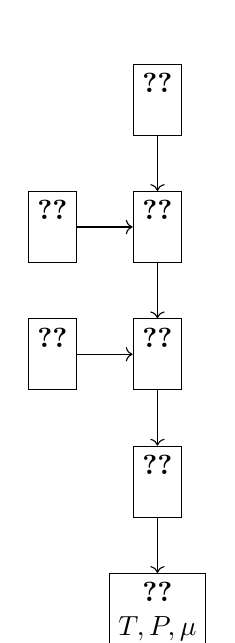
\begin{tikzpicture}[node distance=20pt]
        \node[draw, align=center]                        (chap2)   {第\ref{chap2}章\\经典理想气体简介};
        \node[draw, align=center, below=of chap2]                         (chap4)  {第\ref{chap4}章\\理想气体的位形熵};
        \node[draw, align=center, left=of chap4]                        (chap3)  {第\ref{chap3}章\\离散概率理论};
        \node[draw, align=center, below=of chap4]     (chap6)  {第\ref{chap6}章\\理想气体的能量熵};
        \node[draw, align=center, left=of chap6]                   (chap5)  {第\ref{chap5}章\\连续概率理论};
        \node[draw, align=center, below=of chap6]  (chap7)     {第\ref{chap7}章\\经典理想气体与实际气体的完整熵};
        \node[draw, align=center, below=of chap7]  (chap8)     {第\ref{chap8}章\\$T,P,\mu$与其和熵的关系};

        \draw[->] (chap2) -- (chap4);
        \draw[->] (chap3) -- (chap4);
        \draw[->] (chap4) -- (chap6);
        \draw[->] (chap5) -- (chap6);
        \draw[->] (chap6) -- (chap7);
        \draw[->] (chap7) -- (chap8);

      \end{tikzpicture}
      \caption{第一部分概览}
    \end{figure}
     
    
    \begin{comment}
    \begin{figure}[H]
        \centering
        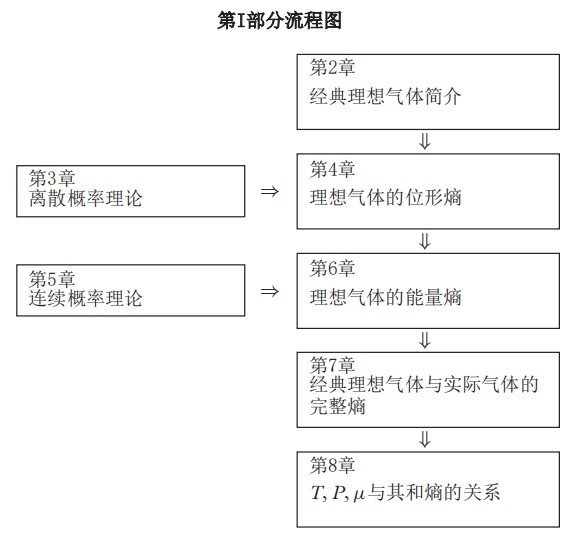
\includegraphics{2-1.jpg}
        \caption{第一部分概览}
    \end{figure}
\end{comment}
    \clearpage
    \section{离散概率理论}
    \label{chap3}
    
    \textit{初始状态一直存在的概率通常很小。系统将从这种状态演变为更可能的状态,直到达到最可能的状态,即热平衡状态。如果我们将其应用于第二定律,我们便可以用这种状态的概率来确定那个通常被称为熵的量。
    \\\rightline{路德维希·玻尔兹曼,1877}}
    \subsection{什么是概率?}\label{sec3.1}
    概率的定义问题重重,以至于在统计学内部引发了类似于宗教战争的事件。其内部有两个基本派系:频率学派(Frequentists)和贝叶斯派(Bayesians)。

    要理解为什么概率的定义会成为一个难题,请考虑一个有$N$次试验的情况,根据某种标准,每一次试验的结果可能是成功或失败。如果$N_s$是成功的次数,那么$N_s/N$被称为这些试验的成功频率。

    频率学派通过无限次试验中成功频率的极限来定义概率,

    \begin{equation}
        p=\lim_{n \to \infty}  \frac{N_s}{N}.
    \end{equation}

    这一定义看起来既精确又客观。事实上,在许多物理文本中,这就是\textit{唯一}的定义。但主要的问题是,人类可用的时间有限,因此根据频率学派的定义,我们永远无法确定任何事情发生的可能性。贝叶斯概率为这一难题提供了解决方案。

    贝叶斯派概率是基于托马斯·贝叶斯(英国数学家、长老会牧师,1702-1761)的工作。贝叶斯派将概率定义为一个人对基于手头证据,对实验结果的知识描述。

    贝叶斯概率定义的一大优点是,它为以下陈述给出了明确的含义:“质子的质量是    $1.672621637(83)×10^{−27}\\kg$”,其中“(83)”称为最后一位的不确定度。“(83)”是什么意思?
    当然,质子的质量是一个明确的数字,在不同的实验中不会出现不同的值。尽管如此,“(83)”作为我们对质子质量确切值的不确定性的表达,确实有其意义。

    在我看来,我们可以要求的唯一合理的客观性形式是,具有相同信息的两个观察者将得出相同的结论,贝叶斯统计满足这一要求。
    \footnote{这种解释有时被称为“客观贝叶斯概率”,以区别于“主观贝叶斯概率”。一些工作者并不认为贝叶斯形式中的“先验”描述了当前实验之前实验者可用的信息,而是认为它是一种任意的选择。有了这种解释,贝叶斯概率便是主观的,对物理学来说也失去了用途。}

    “概率”一词在统计力学中的用法有所不同。我将其称为“模型概率”(Model probability)。这与频率学派的定义最为密切,因为假设模型概率的具体值是准确已知的,就好像我们有无限多次试验一样。
    当然,我们实际上只有有限次的(不精确的)测量,也正如我们将看到的,我们需要确定大量随机变量(超过$10^{20}$个)得出的概率,所以我们无法直接验证我们对实验的假设。

    模型概率仅假设对平衡状态有效。事实上,我们所有的计算都是在平衡状态下的,除了在第22章我们讨论不可逆性时。尽管我们在介绍热力学,但我们的讨论仅限于平衡态之间的转变过程,主要是因为转变过程本身太难计算。

    假定的模型概率形式通常基于一个似是而非的论点,即本质上相似的事件在平衡状态下的概率相等。

    另一个常见的论点涉及到遍历性(Ergodicity),这是一个附加假设。如果系统的轨迹从相空间中的任意点开始,任意接近相空间中的每个允许的点,则系统是遍历的。该轨迹必然是$6N$维空间的一维子集。
    然后在相空间中经历频率相同的区域会被分配相同的概率。遍历性的论点很流行,但它也有一些弱点。一方面,遍历性本身并不能决定哪些区域将被同样频繁地经历。其次,遍历性仅被证明适用于数量非常有限的系统(其中并不包含理想气体)。
    这样的论证也有一个困难,即其轨迹在整个相空间中遍布需要非常长的时间——这个时间与庞加莱重现时间(Poincaré recurrence time,在第22章会讲到)的数量级类似。
    
    一个尽管还没有被证明适用于一般系统,但是更好的论点,是在相空间中非零区域中的初始概率分布开始的,这是一个更现实的假设。如果这种分布随时间的发展可导致对可观测量的唯一预测,那么它就可用于验证模型概率。它的优点是收敛速度更快,如第22章经典理想气体所示。
    \footnote{一般来说,尽管两者对宏观变量的概率给出了相同的预测,不可逆过程后的概率分布与模型概率并不完全相同。这支持了在进行平衡态计算时使用模型概率的方法。}

    然后,我们可以使用我们假设的模型概率来计算实验的预测结果。如果测量结果与我们的预测一致,我们就可以说我们的模型与实验一致。这并不是说我们的模型概率一定是正确的,我们也将在第22章中看到,许多不同的分布也可以导致相同的预测。然而,与实验的一致性总是令人欣慰的。
    
    统计力学以简单的假设为基础,用模型概率表示,这会导致各种各样的预测与实验非常一致。如何做到这一点是本书的主要主题。

    \subsection{离散随机变量与概率}

    我们从对一套基本事件的定义开始,

    \begin{equation}
        A=\{a_j|j=1,\cdots ,N_A\}
    \end{equation}

    并将每个事件赋予一个概率。随机事件及其概率的组合称为“随机变量”(Random variable)。如果基本事件的数量是可数的,那么这就称为“离散随机变量”(Discrete random variable)。

    对于所有的$a_j$,这些概率必须满足条件:

    \begin{equation}\label{eq3.3}
        0\leq P(a_j) \leq 1
    \end{equation}

    不可能事件的概率为0,必然事件的概率为1.

    随机事件可能是任何事件:正面反面,红色黑色,等等。如果所有事件都是一个数字,那么随机变量就称为“随机数” (Random Number)。

    定义基本事件为互斥的——一次有且仅有一个事件发生——所以它们的概率也必须满足归一化条件:
    \begin{equation}\label{eq3.4}
        \sum ^{N_A}_{j=1}P(a_j)=1.
    \end{equation}

    为了简化起见,我们会把这个式子经常写成:
    \begin{equation}
    \sum_{a}P(a)=1,
    \end{equation}
    从而忽略基本事件的数量。
    
    \subsection{多维随机变量的概率理论}\label{sec3.3}
    如果每次试验会发生多于一个事件,那么我们就可以用两个或以上的随机事件来描述这种情况。比如说,$A$中的一个事件与$B$中的一个事件都会发生:

    \begin{equation}
    B=\{b_k|k=1,\cdots ,N_B\}
    \end{equation}

    那么,我们就可以定义联合概率$P(a_j,b_k)$,或更简单地来说,$P(a,b)$,他们必须满足:

    \begin{equation}
        0\leq P(a,b)\leq 1
    \end{equation}
    和:
    \begin{equation}
        \sum_a\sum_b P(a,b)=1
    \end{equation}
    
    \subsubsection{边缘概率与条件概率}\label{sec3.3.1}
    当然,我们如果已知$P(a,b)$,便可以获得$A$或$B$单独的知识。$A$的边缘概率(Marginal Probability)的定义为:
    \begin{equation}\label{eq3.9}
        P_A(a)=\sum_bP(a,b)
    \end{equation}
    对于$P_B(b)$也类似。边缘概率一个很好的性质是它们自动满足公式(\ref{eq3.3})与(\ref{eq3.4})所表示的恒正与归一化性质。
    其被称为边缘概率是因为它可以在概率表的边缘计算得到。表(\ref{table3.1})给出了两个双值随机变量的示例。
    \begin{table}[H]
        \centering
        \caption{\textit{一个独立的随机变量的例子:事件A(标为3和4)被列在左边一列,事件B(标为1和2)列在最上面一列。概率的值体现在中间四格中。边缘包含边缘概率,同公式(\ref{eq3.9})。}}
        \label{table3.1}
        {%
        \begin{tabular}{c|c|c|c}
        \hline
        \multicolumn{1}{c|}{$A\backslash B$} & \multicolumn{1}{c|}{1}   & \multicolumn{1}{c|}{2}   & \multicolumn{1}{c}{$P_A(a)$} \\ \hline
        \multicolumn{1}{c|}{3}   & \multicolumn{1}{c|}{1/2} & \multicolumn{1}{c|}{1/4} & \multicolumn{1}{c}{3/4}    \\ \hline
        4                        & 1/6                      & 1/12                     & 1/4                        \\ \hline
        $P_B(b)$                   & 2/3                      & 1/3                      & 1                          \\ \hline
        \end{tabular}
        }
        \end{table}
    条件概率是在事件$b$发生的情况下,事件$a$发生的概率。其记为$P(a|b)$,且与$A$和$B$同时发生的全概率有关:

    \begin{align}
    P(a,b)&=P(a|b)P_B(b)\label{eq3.10}\\
        &=P(b|a)P_A(a).\label{eq3.11}
    \end{align}
    如果$P_B(b)\neq 0$,那么条件概率$P(a|b)$可写为
    \begin{equation}
    P(a|b)=\frac{P(a,b)}{P_B(b)}.
    \end{equation}
    组合公式(\ref{eq3.10})与(\ref{eq3.11})可以得到贝叶斯定理:
    \begin{equation}\label{eq3.13}
    P(a|b)=\frac{P(b|a)P_A(a)}{P_B(b)}
    \end{equation}
    我们会在第\ref{sec5.5}节讨论贝叶斯定理的结果。
    \subsubsection{独立变量}
    一个尤其有趣的情况是当概率分布可以写作乘积形式时:
    \begin{equation}\label{eq3.14}
        P(a,b)=P_A(a)P_B(b)
    \end{equation}

    当公式(\ref{eq3.14})成立时,这两个随机变量被称为独立的(Independent)。因为若$P_B(b)\neq 0$,条件概率$P(a|b)$就与$b$无关,
    \begin{equation}
        P(a|b)=\frac{P(a,b)}{P_B(b)}=\frac{P_A(a)P_B(b)}{P_B(b)}=P_A(a)
    \end{equation}
    并且$P_(b|a)$也与$a$无关。
    
    表(\ref{table3.1})给出了一个独立随机变量的例子,表(\ref{table3.2})给出了一个非独立随机变量的例子。
    \begin{table}[H]
        \centering
        \caption{\textit{一个非独立的随机变量的粒子。本表与表(\ref{table3.1})的配置相同。}}
        \label{table3.2}
        {%
        \begin{tabular}{c|c|c|c}
        \hline
        \multicolumn{1}{c|}{$C\backslash D$} & \multicolumn{1}{c|}{1}   & \multicolumn{1}{c|}{2}   & \multicolumn{1}{c}{$P_C(c)$} \\ \hline
        \multicolumn{1}{c|}{3}   & \multicolumn{1}{c|}{0.5} & \multicolumn{1}{c|}{0.25} & \multicolumn{1}{c}{0.75}    \\ \hline
        4                        & 0.1                      & 0.15                     & 0.25                        \\ \hline
        $P_D(d)$                   & 0.6                      & 0.4                      & 1                          \\ \hline
        \end{tabular}
        }
        \end{table}

    \subsubsection{两两独立与相互独立}
    如果我们有两个以上变量,那么这组随机变量可能满足两种独立性:两两独立或相互独立。

    两两独立意味着任何\textit{一对}随机变量可以写作单个随机变量边缘概率的积。

    相互独立意味着任一\textit{子集}的随机变量可以写作单个随机变量边缘概率的积。
    
    很明显,相互独立意味着两两独立。但反之是否正确留待本章习题讨论\footnote{译者注:见习题(\ref{prob3.2})}。

    \subsection{随机数与随机变量的函数}\label{sec3.4}
    给定任意随机变量$A=\{a_j|j=1,\cdots ,N_A\}$,我们可以在这个基本事件的集合上定义一个数值函数,$F=\{F(a_j)|j=1,\cdots ,N_A\}$。这个随机数的集合$F$,与它们的概率一起,也是一个随机数。

    如果我们引入克罗内克$\delta$函数(Kronecker delta function):

    \begin{equation}
    \delta_{x,y}=\left\{
        \begin{aligned}
        1\quad x=y \\
        0\quad x\neq y 
        \end{aligned}
        \right.
    \end{equation}
    那么我们就可以简洁地将$F$的概率分布表示出来:
    \begin{equation}\label{eq3.17}
        P_F(f)=\Sigma_a \delta_{f,F(a)}P_A(a)
    \end{equation}
    举一个简单的例子,我们考虑一个可以取三个值-1, 0和1的随机变量,其概率为$P_A(-1)=0.2$, $P_A(0)+0.3$和$P_A(1)+0.5$。定义函数$F(a)=|a|$,故$F$只能取0或1.那么从式(\ref{eq3.17})可以得到概率$P_F(f)$,
    \begin{equation}
        \begin{aligned}
            P_F(0)&=\sum^1_{a=-1}\delta_{0,F(a)}P_A(a)\\
            &=\delta_{0,F(-1)}P_A(-1)+\delta_{0,F(0)}P_A(0)+\delta_{0,F(1)}P_A(1)\\
            &=0+P_A (0)+0=0.3
        \end{aligned}
    \end{equation}
    \begin{equation}
        \begin{aligned}
            P_F(1)&=\sum^1_{a=-1}\delta_{1,F(a)}P_A(a)\\
            &=\delta_{1,F(-1)}P_A(-1)+\delta_{1,F(0)}P_A(0)+\delta_{1,F(1)}P_A(1)\\
            &=P_a(-1)+0+P_A(1)=0.2+0.5=0.7
        \end{aligned}
    \end{equation}
    我们也可以使用$\delta$函数来表达任何以随机数组合而成的新复合随机数。例如,如果$X$和$Y$是随机数,而$G(x,y)$是任意函数,我们可以定义一个新的随机数$Z$。
    $Z$的概率分布以$X$和$Y$所有组合之和给出,并使用$\delta$函数来找出与特定$Z$相对应的组合。
    \begin{equation}\label{eq3.20}
        P_Z(z)=\sum_x\sum_y\delta_{z,G(x,y)}P(x,y)
    \end{equation}
    这里需要警告的是,式(\ref{eq3.20})中求和的范围被省略了。但求和的唯一难点就在于记住这些范围。因为这些范围在连续分布的求解中也十分重要,我们在此给出掷两个骰子,并求其点数之和的概率分布的简单例子。
    \subsubsection*{例子:两个骰子点数之和的概率}
    我们在此假设骰子是均匀的(Honest)。在物理题目中他们经常如此,但在实际生活中却不然。令
    $X=\{x|x=1,2,3,4,5,6\}$作为表示第一个骰子的结果的随机数,$Y$为表示第二个骰子对应结果的随机数。和为$S=X+y$。$S$的值可以从2取到12.
    因为所有基本事件的概率相同,
    \begin{equation}
        P(x,y)=P_X(x)P_y(y)=(\frac{1}{6})(\frac{1}{6})=\frac{1}{36}
    \end{equation}
    那么式(\ref{eq3.20})就变为
    \begin{equation}\label{eq3.22}
        P(s)=\frac{1}{36}\sum^6_{x=1}\sum^6_{y=1}\delta_{s,x+y}
    \end{equation}
    先对$y$求和。其值决定于是否对于某些$y$值,$s=x+y$成立,或者等价于是否$s-x$处于区间$[1,6]$中
    \begin{equation}
        \sum^6_{y=1}\delta_{s,x+y}=\left\{
        \begin{aligned}
        1\quad &1\leq s-x\leq 6.\\
        0\quad & \mbox{其他}
        \end{aligned}
        \right.
    \end{equation}
    这对于对$x$求和给出了两个限制。只有满足$x\leq s-1$和$x\geq s-6$的$x$会对结果有贡献。这些限制还需要加上求和号上$x\leq 6$与$x \geq 1$的限制。
    因为这四个不等关系都需要满足,我们对每一种情况都需要有更严格的不等关系。哪种不等关系更严格取决于$s$的大小,列于表(\ref{table3.3})中。
    
    对于$s\leq 7$,$x$的下限为$1$,上限为$s-1$.于$s\geq 7$,$x$的下限为$s-6$,上限为$6$.这个和可以显式地表示出来,
    \begin{equation}
        P(s)=\left\{
            \begin{aligned}
            &\sum^{s-1}_{x=1}\frac{1}{36}=\frac{s-1}{36}\quad s\leq 7 \\
            &\sum^{6}_{x=s-6}\frac{1}{36}=\frac{13-s}{36}\quad s\geq 7.
            \end{aligned}
            \right.
    \end{equation}
    
    尽管$X$与$Y$的概率分布均是均匀的,但$S$的概率分布却不是。这是个很重要的结果。尽管我们通常会假设大多数微观量的基本概率分布是均匀的,但我们会看到宏观观测值的分布将非常快速地达到峰值。
    \begin{table}[H]
        \centering
        \caption{\textit{当使用式(\ref{eq3.22})时第二个求和的上下限}}
        \label{table3.3}
        {%
        \begin{tabular}{ccc}
        \hline
               \quad        & 下限      & 上限      \\ \hline
        求和的限制:         & x $\geq$ 1   & x $\leq$ 6   \\ \hline
        $\delta$函数导致的限制: & x $\geq$ s−6 & x $\leq$ s−1 \\ \hline
        s$\leq$7下更加严格的限制: & x $\geq$ 1   & x $\leq$ s−1 \\ \hline
        s$\geq$7时更加严格的限制: & x $\geq$ s−6 & x $\leq$ 6   \\ \hline
        \end{tabular}%
        }
        \end{table}
    必须要承认的一点是,有更简单的方法来进行两个骰子之和的概率分布的数值计算,特别是当需要数值解的时候。式(\ref{eq3.20})对于计算机来说十分方便,因为克罗内克$\delta$函数就对应着"IF"语句。
    然而,我们将有充足的机会将刚才描述的最简单的方法应用于实际问题。选择本节中的示例的一个原因是,正确的答案很容易理解,而这便使得这个方法更加易懂。
        
    \subsection{平均值,方差与标准差}
    由随机变量$A$所定义的$F(A)$的平均值,由以下式子给出:
    \begin{equation}
        \langle{F}\rangle\equiv\sum_aF(a)P_A(a).
    \end{equation}
    与其类似,$F$的$n$阶矩(nth moment)可以定义为:
    \begin{equation}
        \langle{F^n}\rangle\equiv\sum_aF(a)^nP_A(a).
    \end{equation}
    
    $n$阶中心矩(nth central moment)由减去平均值再求$n$次方所定义:
    \begin{equation}
        \langle{(F-\langle{F}\rangle)^n}\rangle\equiv\sum_a(F(a)-\langle{F}\rangle)^nP_A(a).
    \end{equation}
    
    $2$阶矩被称为方差$\sigma^2$,在统计分析中有着很重要的作用:
    \begin{equation}
        \sigma^2=\langle{(F-\langle{F}\rangle)^2}\rangle=\sum_a(F(a)-\langle{F}\rangle)^2P_A(a).
    \end{equation}
    其也可以写作:
    \begin{equation}
        \sigma^2=\langle{(F-\langle{F}\rangle)^2}\rangle=\langle{F^2}\rangle-\langle{F}\rangle^2.
    \end{equation}
    方差的开方也叫作标准差,
    \begin{equation}
        \sigma\equiv\sqrt{\langle{F^2}\rangle-\langle{F}\rangle^2}.
    \end{equation}
    标准差经常被用于测量概率分布的宽度。

    \subsection{相关函数}
    假设我们有两个随机数$A$和$B$,也已知他们的联合概率分布$P(A,B)$,与定义在这两个随机数上的函数$F(A)$,$F(B)$。$F$和$G$是随机数,且我们可以探究它们之间的关系。特别地,我们可以定义相关函数$f_{FG}$,
    \begin{equation}
        f_{FG}=\langle{FG}\rangle-\langle{F}\rangle\langle{G}\rangle.
    \end{equation}
    
    当$F$与$G$相互独立,我们应该得到相关函数等于$0$的结论,实际上也是这样的:
    \begin{equation}
        \begin{aligned}
            f_{FG}=&\sum_a\sum_bF(a)G(b)P(a,b)\\
            &-\sum_aF(a)P_A(a)\sum_bG(b)P_B(b)\\
            =&\sum_a\sum_bF(a)G(b)P_A(a)P_B(b)\\
            &-\sum_aF(a)P_A(a)\sum_bG(b)P_B(b)\\
            =&0.
        \end{aligned}
    \end{equation}
    
    \subsection{一组独立的随机数}\label{sec3.7}
    给定一组随机数$\{F_j|j=1,\cdots ,N\}$,我们经常对于另一组由它们之和组成的随机数感兴趣:
    \begin{equation}
        S=\sum^N_{j=1}F_j
    \end{equation}

    我们很容易计算随机数$S$的平均值,就是每个随机数的平均值之和:
    \begin{equation}
        \langle{A}\rangle=\langle{\sum^N_{j=1}F_j}\rangle=\sum^N_{j=1}\langle{F_j}\rangle
    \end{equation}

    如果这些随机数两两独立,我们便可计算方差与标准差:
    \begin{equation}
        \begin{aligned}
            \sigma_{S}^{2} & \equiv\left\langle S^{2}\right\rangle-\langle S\rangle^{2} \\
            &=\sum_{j=1}^{N} \sum_{k=1}^{N}\left\langle F_{j} F_{k}\right\rangle-\sum_{j=1}^{N}\left\langle F_{j}\right\rangle \sum_{k=1}^{N}\left\langle F_{k}\right\rangle \\
            &=\sum_{j=1}^{N} \sum_{k=1(k \neq j)}^{N}\left\langle F_{j}\right\rangle\left\langle F_{k}\right\rangle+\sum_{j=1}^{N}\left\langle F_{j}^{2}\right\rangle-\sum_{j=1}^{N}\left\langle F_{j}\right\rangle \sum_{k=1}^{N}\left\langle F_{k}\right\rangle \\
            &=\sum_{j=1}^{N}\left(\left\langle F_{j}^{2}\right\rangle-\left\langle F_{j}\right\rangle^{2}\right) \\
            &=\sum_{j=1}^{N} \sigma_{j}^{2} .
            \end{aligned}
    \end{equation}
    在这个推导中,$\sigma_j^2$代表第$j$个随机数的方差。我们可以看到,一组\textit{两两独立}的随机数的和的方差就是他们方差的和。

    如果一组随机数$F_j$都有相同的平均数和方差,那么这个式子就可以进一步简化。如果对于所有的$j$都有$\langle{F_j}\rangle\langle{F}\rangle$,那么:
    \begin{equation}
        \langle{S}\rangle=\sum^N_{j=1}\langle{F_j}\rangle=N\langle{F}\rangle
    \end{equation}
    类似地,如果对于所有的$j$都有$\sigma_j^2=\sigma^2$,那么
    \begin{equation}
        \sigma_S^2=\sum^N_{j=1}\sigma_j^2=N\sigma^2
    \end{equation}

    注意$S$的标准差与根号下变量数目呈正比关系:
    \begin{equation}
        \sigma_S=\sigma \sqrt{N}
    \end{equation}
    另外,相对标准差与根号下变量数目呈正比关系:
    \begin{equation}
        \frac{\sigma_S}{\langle{S}\rangle}=\frac{\sigma\sqrt{N}}{N\langle{F}\rangle}=\frac{\sigma}{\langle{F}\rangle\sqrt{N}}
    \end{equation}
    也许有人会说这是概率论在统计力学中最重要的结论。对于统计力学的许多应用场合中,$N$的恰当值是$10^{20}$或更大,所以宏观量的相对不确定性的数量级基本是$10^{-10}$或更小。这比大多的实验误差要小得多,所以预测的结果基本没有不确定性。

    \subsection{二项分布}\label{sec3.8}
    一种特别重要的情况是$N$个独立且分布相同的随机数$\{F_j\}$,每个都有$p$的概率取1,有$1-p$的概率取0.扔硬币便是一个例子,硬币可能是均匀的($p=0.5$)或不均匀的($p\neq 0.5$)。

    每个随机数的平均值与方差很容易计算:$\langle{F}\rangle=p$与$\sigma^2=p(1-p)$。他们之和
    \begin{equation}
        S=\sum^N_{j=1}F_j
    \end{equation}
    的平均值和方差便是:
    \begin{equation}\label{eq3.41}
        \langle{S}\rangle=pN
    \end{equation}
    与:
    \begin{equation}\label{eq3.42}
        \sigma_S^2=p(1-p)N.
    \end{equation}
    标准差为:
    \begin{equation}\label{eq3.43}
        \sigma_S=\sqrt{p(1-p)N}
    \end{equation}
    相对标准差为:
    \begin{equation}
        \frac{\sigma_S}{\langle{S}\rangle}=\frac{\sqrt{p(1-p)N}}{pN}=\sqrt{\frac{1-p}{pN}}.
    \end{equation}
    \subsubsection{二项分布的导出}\label{sec3.8.1}
    我们可以进一步推导随机数之和的概率分布$P(S)$。此结果对于经典理想气体的分析极为重要。

    某特定的含有$n$个随机变量的子集取值为1,其余$N-n$个随机变量取0的概率很容易得出:
    \begin{equation}\label{eq3.45}
        p^n(1-p)^{N-n}
    \end{equation}

    为了完成计算,我们只需要确定随机变量在取给出个数的1和0下的排列数。这等同于$N$个不同物体放在两个箱子中,第一个箱子放$n$个,第二个箱子放$N-n$个。

    为了计算排列的个数,先考虑$N$个物体顺序排列的方法数,因为$N$个物体中任意一个都可以排第一位,$N-1$个物体中任意一个都可以排第二位等等,所以共有$N!=N(N-1)(N-2)\cdots 2\cdot 1$种排法。

    在将物品放入两个箱子的问题中,每个箱子中物体的顺序并不重要。故因为第一个箱子内部中的重复,我们必须除以$n!$,因为第二个箱子中的重复,我们必须除以$(N-n)!$。最终排列个数被称为二项式系数,并有自己的标准符号:
    \begin{equation}\label{eq3.46}
    \binom{N}{n} = \frac{N!}{n!(N-n)!}
    \end{equation}
    将其乘以式(\ref{eq3.45})便给出了二项分布公式:
    \begin{equation}\label{eq3.47}
        P(n|N)=\frac{N!}{n!(N-n)!}p^n(1-p)^{N-n}=\binom{N}{n}p^n(1-p)^{N-n}.
    \end{equation}

    二项分布这个名字由二项式定理得来,这个定理表明对于任意的$p$与$q$,
    \begin{equation}
        (p+q)^N=\sum^N_{n=0}\frac{N!}{n!(N-n)!}p^nq^{N-n}=\sum^N_{n=0}\binom{N}{n}p^nq^{N-n}
    \end{equation}
    取$q=1-p$可以证明式(\ref{eq3.47})中的二项式分布是归一化的。
    \subsubsection{二项式系数的有用性质}
    尽管对于二项式系数的推导看上去十分直接,$N!$关于$N$的增长快到我们很难直接应用定义。例如,某广泛使用的表格软件在$N=171$时便溢出了,我的手持计算器甚至无法计算$N=70$.

    另一方面,二项式系数本身并不并不随$N$快速增长。下面的性质由式(\ref{eq3.46})直接得出,它们可以使我们摆脱数值计算的困扰直接得到较大$N$时的二项式系数。
    \begin{align}
    \binom{N}{0}=\binom{N}{N}=1\\
    \binom{N-1}{n}+\binom{N-1}{n-1}=\binom{N}{n}\\
    \binom{N}{n+1}=\frac{N-n}{n+1}\binom{N}{n}
    \end{align}
    
    这些性质的证明留做练习。

    \subsection{二项分布的高斯近似}\label{sec3.9}
    对于固定的$p$值,和很大的$N$值,二项分布可以用高斯分布来近似。这被称为中心极限定理(Central limit theorem)。我们不会在此证明,但我们会展示如何恰当地确定高斯分布中的参数。

    考虑高斯函数:
    \begin{equation}
    g(x)=\frac{1}{\sqrt{2 \pi \sigma^{2}}} \exp \left[-\frac{\left(x-x_{0}\right)^{2}}{2 \sigma^{2}}\right]
    \end{equation}

    其平均数与模(最大值位置)相同:
    \begin{equation}
        \langle x\rangle=x_{0}=x_{\max }
    \end{equation}

    方差由二阶矩给出:
    \begin{equation}
        \begin{aligned}
            \left\langle\left(x-x_{0}\right)^{2}\right\rangle &=\frac{1}{\sqrt{2 \pi \sigma^{2}}} \int_{-\infty}^{\infty}\left(x-x_{0}\right)^{2} \exp \left[-\frac{\left(x-x_{o}\right)^{2}}{2 \sigma^{2}}\right] d x \\
            &=\frac{1}{\sqrt{2 \pi \sigma^{2}}} \int_{-\infty}^{\infty} y^{2} \exp \left[-\frac{y^{2}}{2 \sigma^{2}}\right] d y \\
            &=\frac{1}{\sqrt{2 \pi \sigma^{2}}} \frac{1}{2} \sqrt{\pi}\left[2 \sigma^{2}\right]^{3 / 2} \\
            &=\frac{1}{\sqrt{2 \pi \sigma^{2}}} \sqrt{\pi} \sqrt{2 \sigma^{2}} \sigma^{2} \\
            &=\sigma^{2}
            \end{aligned}
    \end{equation}
    
    现在,寻找一个二项分布的高斯近似便很简单了。因为平均值与方差可以从式(\ref{eq3.41})与式(\ref{eq3.42})得出:
    \begin{equation}
        \langle{n}\rangle=pN
    \end{equation}
    与:
    \begin{equation}
        \sigma^2=p(1-p)N
    \end{equation}

    具有该平均值与方差的高斯分布可以作为二项分布$n$与$N$充分大时的良好近似。
    \begin{equation}\label{eq3.57}
    P(n \mid N) \approx \frac{1}{\sqrt{2 \pi p(1-p) N}} \exp \left[-\frac{(n-p N)^{2}}{2 p(1-p) N}\right]
    \end{equation}

    多大的$n$与$N$才能称得上是一个好的近似,将留作一个数值练习。

    \subsection{关于高斯积分的一些偏题}\label{sec3.10}
    在$N$大到$10^{20}$时,为了得到一个$N!$的既实用又准确的近似,我们需要使用另一个数学工具:高斯积分。

    高斯积分在统计力学中重要到我们特意在此花一小节来讲述。尽管本节导出的积分公式在很多地方都能找到,但是学统计力学的学生应当能够在不借助外界参考的情况下计算出高斯积分。

    计算下列积分的第一步对于非高斯积分也很有帮助;
    \begin{equation}\label{eq3.58}
        G=\int_{-\infty}^{\infty} e^{-a x^{2}} dx
    \end{equation}
    因为我们有时只需要计算积分关于参数$a$的性质。进行变量代换$y=x\sqrt{a}$,使式(\ref{eq3.58})中的积分无量纲化。
    \begin{equation}
        G=\frac{1}{\sqrt{a}} \int_{-\infty}^{\infty} e^{-y^{2}} dy
    \end{equation}
    注意其与参数$a$的关系只在于前面的因子。

    为了计算这个无量纲的积分,我们将其平方,并将结果写作一个二重积分:
    \begin{equation}
        \begin{aligned}
            G^{2} &=\frac{1}{\sqrt{a}} \int_{-\infty}^{\infty} e^{-x^{2}} d x \frac{1}{\sqrt{a}} \int_{-\infty}^{\infty} e^{-y^{2}} d y \\
            &=\frac{1}{a} \int_{-\infty}^{\infty} \int_{-\infty}^{\infty} e^{-\left(x^{2}+y^{2}\right)} d x d y \\
            &=\frac{1}{a} \int_{0}^{\infty} e^{-r^{2}} 2 \pi r d r \\
            &=\frac{\pi}{a}\left[-e^{-r^{2}}\right]_{0}^{\infty}=\frac{\pi}{a} .
            \end{aligned}
    \end{equation}
    高斯积分的值便是:
    \begin{equation}\label{eq3.61}
        \int_{-\infty}^{\infty} e^{-a x^{2}} d x=\sqrt{\frac{\pi}{a}}
    \end{equation}

    \subsection{\texorpdfstring{对于$N!$的斯特林近似}{对于N!的斯特林近似}}\label{sec3.11}
    就像之前所述,使用二项分布的一大难点在于当$N$较大的时候,$N!$会变得极大。对于$N=25$,$N!\approx 1.6\times 10^{25}$,而我们需要考虑$N$为$10^{20}$或更大的情况!我们也需要对于概率分布进行微分与积分,而积的表示也带来了不便。

    这个问题的解决方法是斯特林近似(Stirling's approximation)。它对于大数有效——正是我们想要讨论的情况。我们会从最简单的开始,讨论斯特林近似的各阶情况。
    \subsubsection{斯特林近似的最简单形式}
    考虑将$lnN!$近似为一个积分:
    \begin{equation}
        \ln N !=\ln \left(\prod_{n=1}^{N} n\right)=\sum_{n=1}^{N} \ln (n) \approx \int_{1}^{N} \ln (x) d x=N \ln N-N+1
    \end{equation}
    这也等同于近似
    \begin{equation}\label{eq3.63}
        N ! \approx N^{N} \exp (1-N)
    \end{equation}
    \subsubsection{斯特林近似的一个更佳的形式}
    一个更好的近似可以通过$N!$的准确积分形式获得:
    \begin{equation}\label{eq3.64}
        N !=\int_{0}^{\infty} e^{-x} x^{N} d x
    \end{equation}
    式(\ref{eq3.64})的正确性可以由归纳法得到。对于$N=0$时明显正确,因为$0!=1=\int^{\infty}_0e^{-x}dx$。如果式子对$N$正确,那么通过分部积分,我们也可以证明对$N+1$成立,
    \begin{equation}
        \begin{aligned}
            (N+1) ! &=\int_{0}^{\infty} e^{-x} x^{N+1} d x \\
            &=\left[-e^{-x} x^{N+1}\right]_{0}^{\infty}-\int_{0}^{\infty}\left(-e^{-x}(N+1) x^{N}\right) d x \\
            &=(N+1) N !
            \end{aligned}
    \end{equation}
    
    注意到式(\ref{eq3.64})中的积分在$N$较大时快速达到峰值,故我们可以使用最速下降法(Method of steepest descent)对其进行近似。其包含使用以下形式的高斯公式对被积函数进行近似:
    \begin{equation}
        g(x)=A \exp \left[-\frac{\left(x-x_{0}\right)^{2}}{2 \sigma^{2}}\right]
    \end{equation}
    其中,$A,x_0,\sigma$都是待确定的参数。

    我们可以通过取一阶导等于0的方式确定式(\ref{eq3.64})的最大值位置。对于高斯分布,即:
    \begin{equation}\label{eq3.67}
        \frac{d}{d x} \ln g(x)=\frac{d}{d x}\left[\ln A-\frac{\left(x-x_{0}\right)^{2}}{2 \sigma^{2}}\right]=-\frac{\left(x-x_{o}\right)}{\sigma^{2}}=0
    \end{equation}
    或$x=x_0$。
    通过比较式(\ref{eq3.67}),并使式(\ref{eq3.64})中被积式对数的一阶导等于0,我们便可以找到取最大值的位置$x_0$:
    \begin{equation}
        0=\frac{d}{d x}[-x+N\ln x]=-1+\frac{N}{x}
    \end{equation}
    或$x=x_0=N$.那么函数值的最大值就是式(\ref{eq3.64})中取$x=x_0=N$时的值,即$A=e^{-N}N^N$。

    高斯函数对数的二阶导给出方差的值:
    \begin{equation}
        \frac{d^{2}}{d x^{2}} \ln g(x)=\frac{d}{d x}\left[-\frac{\left(x-x_{0}\right)}{\sigma^{2}}\right]=-\frac{1}{\sigma^{2}}
    \end{equation}
    当使用这种方法计算高斯近似的方差时,被近似函数对数的二阶导应当在$x_0$取值。

    为了得出$\sigma^2$的值,我们取式(\ref{eq3.64})对数的二阶导,并计算其在$x_0$的值。
    \begin{equation}
        -\frac{1}{\sigma^{2}}=\frac{d^{2}}{d x^{2}}[-x+N \ln x]=\frac{d}{d x}\left[-1+\frac{N}{x}\right]=-\frac{N}{x^{2}},
    \end{equation}
    或:
    \begin{equation}
    \sigma^{2}=\frac{x_{0}^{2}}{N}=N
    \end{equation}
    我们可以使用(\ref{sec3.10})节的高斯积分公式:
    \begin{equation}\label{eq3.72}
        N !=\int_{0}^{\infty} e^{-x} x^{N} d x \approx \int_{0}^{\infty} e^{-N} N^{N} \exp \left[-\frac{(x-N)^{2}}{2 N}\right] d x \approx e^{-N} N^{N} \sqrt{2 \pi N}
    \end{equation}
    从表(\ref{table3.4})可以看出,式(\ref{eq3.72})相较式(\ref{eq3.63})有着巨大的提升。
    \begin{mdframed}[backgroundcolor=lightgray,hidealllines=true]
    
        本节中通过高斯函数近似一个快速达到峰值的函数的方法在统计力学中极其普遍,因为我们遇到的很多函数都具有这样的性质。
    \end{mdframed}
    \begin{table}[H]
        \centering
        \caption{\textit{各阶斯特林近似与$N!$准确结果的对比。“斯特林(简单)”即式(\ref{eq3.63}),“斯特林(改进)”即式(\ref{eq3.72}),“高斯帕”即式(\ref{eq3.73})}。}
        \label{table3.4}
        \resizebox{\textwidth}{!}{%
        \begin{tabular}{cccccccc}
        \hline
        N  & N!                 & 斯特林               & 误差    & 斯特林               & 误差      & 斯特林                & 误差       \\
           &                    & (简单)              &       & (改进)              &         & (高斯帕)              &          \\ \hline
        1  & 1                  & 1                 & $0\%$   & 0.922             & $-7.79\%$ & 0.996              & $-0.398\%$ \\
        2  & 2                  & 1.47              & $-26\%$ & 1.919             & $-4.05\%$ & 1.997              & $-0.132\%$ \\
        3  & 6                  & 3.65              & $-39\%$ & 5.836             & $-2.73\%$ & 5.996              & $-0.064\%$ \\
        4  & 24                 & 12.75             & $-47\%$ & 23.506            & $-2.06\%$ & 23.991             & $-0.038\%$ \\
        5  & 120                & 57.24             & $-52\%$ & 118.019           & $-1.65\%$ & 119.970            & $-0.025\%$ \\
        10 & 3628800            & 1234098           & $-66\%$ & 3598694           & $-0.83\%$ & 3628559            & $-0.007\%$ \\
        20 & $2.43\times 10^{18}$ & $5.87\times10^{17}$ & $-76\%$ & $2.43\times10^{18}$ & $-0.42\%$ & $1.43\times 10^{18}$ & $-0.002\%$ \\ \hline
        \end{tabular}%
        }
        \end{table}
        
    \subsubsection{高斯帕近似}
    最后,我们给出一个斯特林近似的变体——高斯帕(Gosper)近似\footnote{引用自\href{http://mathworld.wolfram.com/StirlingsApproximation.html}{http://mathworld.wolfram.com/StirlingsApproximation.html}}
        \begin{equation}\label{eq3.73}
            N ! \approx e^{-N} N^{N} \sqrt{\left(2 N+\frac{1}{3}\right) \pi}
        \end{equation}
    表(\ref{table3.4})显示出高斯帕近似在非常小的$N$下也给出了很好的近似。
    \subsubsection{斯特林公式的应用}
    在统计力学的应用中,我们经常对于概率分布的对数,以及$lnN!$感兴趣。这就导致斯特林近似中最简单的形式反而是最常用的,尽管从表(\ref{table3.4})中可以看出,当$N$很大时,其对于$N!$的近似很差。

    从高斯帕近似来看,我们有着十分准确的公式来表达$N!$:
    \begin{equation}\label{eq3.74}
        \ln N ! \approx N \ln N-N+\frac{1}{2} \ln \left[\left(2 N+\frac{1}{3}\right) \pi\right]
    \end{equation}

    在统计力学中,我们对于很大的$N$最感兴趣,$N$的取值从$10^{12}$到$10^{24}$左右。那么使用斯特林近似的最简单形式\((lnN!\approx NlnN-N)\)的误差即为$1/N$,对于“小”到$10^{12}$的$N$也是可以忽略的。对于$N=10^{24}$,$lnN!\approx NlnN-N$是物理学中最为准确的近似之一。

    \subsection{应用斯特林近似的二项分布}
    因为式(\ref{eq3.74})中的最后一项对于很大的$N$来说可以忽略,故最常用的近似是只取前两项。如果我们使用斯特林公式的这种形式,我们就可以将式(\ref{eq3.47})中的二项分布表示为一个恰当但又高度准确的形式:
    \begin{equation}
        P(n \mid N)=\frac{N !}{n !(N-n) !} p^{n}(1-p)^{N-n}
    \end{equation}
    \begin{equation}\label{eq3.76}
        \begin{aligned}
            \ln P(n \mid N) \approx & N \ln N-n \ln n-(N-n) \ln (N-n) \\
            &+n \ln p+(N-n) \ln (1-p)
            \end{aligned}
    \end{equation}
    注意式(\ref{eq3.74})中斯特林近似的第二项在式(\ref{eq3.76})中被消去。

    对于二项分布应用斯特林近似有一些好处。我们知道二项分布的峰值很尖锐,且相对宽度很小。我们可以使用斯特林近似来求出峰值的位置,将$n$视为连续变量,且在式(\ref{eq3.47})中将概率的对数关于$n$求导等于0,
    \begin{equation}
        \frac{\partial}{\partial n} \ln P(n \mid N)=0
    \end{equation}
    或:
    \begin{equation}
        \begin{aligned}
            0=& \frac{\partial}{\partial n}[\ln N !-\ln n !-\ln (N-n) !+n \ln p+N-n \ln (1-p)] \\
            =& \frac{\partial}{\partial n}[N \ln N-N-n \ln n-n-(N-n) \ln (N-n)-(N-n)\\
            &+n \ln p+N-n \ln (1-p)] \\
            =&-\ln n+\ln (N-n)+\ln p-\ln (1-p)
            \end{aligned}
    \end{equation}
    本式导出了有关最大概率位置$n_0$的关系:
    \begin{equation}
        \frac{n_{o}}{N-n_{o}}=\frac{p}{1-p}
    \end{equation}
    有解:
    \begin{equation}
        n_0=pN.
    \end{equation}
    这就意味着斯特林近似给出峰值位置就是\textit{准确}值$\langle{n}\rangle=pN$.
    \subsection{多项分布}\label{sec3.13}
    二项分布一个很重要的推广是多项分布。在此,我们考虑$N_T$个粒子分到$M\geq2$个盒子中,这些盒子标为$j=1,\ldots,M.$

    每一个粒子的分配方式与其他粒子都独立。如果每个粒子分到第$j$个盒子的概率为$p_j$,那么一组特定的粒子被分到第$j$个盒子的概率为:
    \begin{equation}
        \prod_{j=1}^{M} p_{j}^{N_{j}}
    \end{equation}
    这是式(\ref{eq3.45})的推广。这个式子必须乘以在$N_T$中选择$N_j$个粒子的方法数。这个方法与(\ref{sec3.8.1})小节中的叙述相对应。对于$N_T$个粒子,一共有$N_T!$种排列方法。将它们分到$M$个盒子中,每个盒子有$N_j$个粒子,其中$\sum_jN_j=N_t$。
    每个盒子中粒子的排列顺序无关紧要,所以我们对于每个盒子$j$都需要除以$N_j!$。结果便是多项分布:
    \begin{equation}\label{eq3.82}
        P\left(\left\{N_{j}\right\}\right)=\left(\frac{N_{T} !}{\prod_{j=1}^{M} N_{j} !}\right) \prod_{j=1}^{M} p_{j}^{N_{j}}
    \end{equation}

    将其应用于理想气体,我们假设某个特定的粒子在体积$V_j$中被找到的概率与$V_j$成正比。如果总体积为$V_T=\sum_jV_J$,那么概率为$V_j/V_T$。代入式(\ref{eq3.82})得到:
    \begin{equation}\label{eq3.83}
        P\left(\left\{N_{j}\right\}\right)=\left(\frac{N_{T} !}{\prod_{j=1}^{M} N_{j} !}\right) \prod_{j=1}^{M}\left(\frac{V_{j}}{V_{T}}\right)^{N_{j}}=\frac{N_{T} !}{V_{T}^{N_{T}}} \prod_{j=1}^{M}\left(\frac{V_{j}^{N_{j}}}{N_{j} !}\right)^{N_{j}}
    \end{equation}
    这个式子对于下一章非常重要。它其实对于整个统计力学来说都很重要。
    \subsection{习题}
    \subsubsection*{示例程序:掷一个骰子}
    示例程序采用Python 2. \footnote{译者注:在Python 3.3以后,time.clock已被弃用,可以使用time.perf\_counter或time.process\_time来代替。}

    给出的程序首先询问你掷骰子的次数。接着,其在1到6之间任选一个整数,记录其值,并重复,直到其取够你要求的数量。然后其输出柱状图(每个整数取到的次数),告知你程序的运行时间,并退出。

    柱状图对于本章与其他章节中所探究的问题起到十分重要的作用。其仅作为特定实验或模拟过程中对于每个可能结果的次数记录。柱状图的表示相对于列出所有生成的结果更加紧凑。通过简单地将柱状图中的条目除以投掷次数,我们可以得到每个结果的概率估计值。
    
    为了列出所有显示方法,柱状图将以两种格式输出。本程序中计算了运行程序所需的时间,且这将会非常有用。由于“trials”(测试的次数)和“sides”(骰子的面数)都是整数,除法“trials/sides”会截断结果并给出一个整数,这在许多计算机语言中很常见。如果使用Python 3,此除法将生成一个浮点数。
    
    该程序中使用了两个特殊的Python命令:numpy.zeros(sides,int)和random.random()。
    命令\\numpy.zeros(sides,int)位于“模块”numpy中,其在程序的第一行被导入。它生成一个零向量。命令random.random()位于“模块”random中,其在程序的第二行被导入。

    需要输出的文字用双引号或单引号括起来,但引号必须匹配。

    花几分钟时间测试一下这个程序。改一改语句,看看会发生什么。编程的一个好处是你不会把电脑弄坏。

    当你完成一个程序的编写时,使用不同大小的参数运行几次。这样不会花很多时间,但会给出参数对概率分布的大致规律,这便是编程中最有趣的部分了。

    下面的代码属于程序 "OneDie\_PARTIAL.py"。

    \begin{python}
    import numpy
    import random
    from time import clock
    t0 = clock()

    trials = 100
    print " Number of trials = " , trials

    sides = 6
    histogram = numpy.zeros(sides,int)
    print histogram

    j=0
    while j < trials :
        r = int( random . random () ∗ sides )
        histogram[r] = histogram[r] + 1
        j=j+1
    print histogram

    s=0
    while s < sides :
        print s , histogram [s], histogram [s] − trials / sides
        s=s+1
    t1 = clock ()
    print "\n Program time = " , ’% 10.4 f ’ % ( t1 − t0) , " seconds "
    \end{python}
    \textbf{习题3.1}\\
    \textbf{使用计算机掷一个骰子}
    
    在本习题中,你可以修改给出的Python程序(OneDie\_PARTIAL.py),或者从头开始,用任意语言写出你自己的程序。
    \begin{enumerate}
        \item 编写一个程序(或修改给出的程序),计算并输出每面出现次数的柱状图、每面出现次数与总次数的六分之一之差、每面出现的频率、与其和六分之一的差。同时上交你所使用的程序。
        \item 提供程序的一次典型输出。
        \item 使用不同大小的随机整数运行几次,从很小的数(比如10)开始,逐渐增加到一个非常大的数。唯一的限制是,你的程序不应运行超过一秒。(你的时间非常宝贵。)\\
        {\kaishu 这是一个计算机习题。\\所有的答案都应提供数据。}\\请在解答中提交所有的数值数据。
        \item 投掷次数增加时,某面出现的次数与总次数的六分之一的差(绝对值)是增加还是减少?\\(本问与下一问不同。)
        \item 当投掷次数增加时,某面出现的频率(某面出现次数除以总次数)与1/6是否更接近?
    \end{enumerate}
    \textbf{习题3.2}\label{prob3.2}\\
    \textbf{相互独立}

    我们在本章中定义了两两独立的概念。与其相关的概念还有\textit{相互独立}。考虑一组随机变量:
    $$\{A_j|j=1,\cdots,N\}$$
    如果任意包含$n$个随机变量的${A_j}$的子集都满足以下条件,那么就称其相互独立:其边缘概率满足条件:
    \begin{equation}
        P_{i, j, \ldots, n}\left(a_{i}, a_{j}, a_{k}, \ldots, a_{n}\right)=P_{i}\left(a_{i}\right) P_{j}\left(a_{j}\right) P_{k}\left(a_{k}\right) \cdots P_{n}\left(a_{n}\right).
    \end{equation}
    很明显,相互独立意味着两两独立。问题在于,两两独立是否意味着相互独立。

    请提供证明或反例。\\
    \textbf{习题3.3}\label{prob3.3}\\
    \textbf{具有任意面数的骰子}

    假设我们有一个$S$面的骰子,其中$S$为整数,但不一定等于6.可能的结果于是为$\{n|n=1,\cdots,S\}$(或者$\{n|n=0,\cdots,S-1\}$)。假设骰子的所有面都是等可能的,故$P(n)=1/S$。

    因为本题的一部分是计算机习题,故请确保你的数据是由计算机模拟得出的。
    \begin{enumerate}
        \item 平均值,方差,标准差的理论值为多少?将其表示为$S$的函数。结果应该为最简式,而不应含有求和符号。(提示:复习整数和公式与平方和公式可能会有帮助。)
        \item 修改之前的程序,使其用于模拟一个$S$面的骰子,并对特定投掷数输出平均值、方差与标准差。使程序输出理论值,与实际值对于理论值的偏差,方便比较。
        \item 对于两个非常不同的$S$值运行程序。平均值、方差与标准差与你的预测相符吗?(不要让程序运行超过一秒,否则等待程序运行非常浪费时间。)
        \item 尝试不同的投掷次数。为了获得平均值与标准差的\textit{粗糙}估计,你需要多少次投掷?为了获得误差小于$1\%$的结果,你需要多少次投掷?对于平均值与标准差,两者获得小于$1\%$的结果需要的次数相同吗?
    \end{enumerate}
    \textbf{习题3.4}\label{prob3.4}\\
    \textbf{独立性与相关函数}

    我们已经给出,如果随机变量$A$与$B$互相独立,且$F(A)$与$G(B)$是定义在$A,B$上的数值函数,那么:
    \begin{equation*}
        \langle F(A) G(B)\rangle=\langle F(A)\rangle\langle G(B)\rangle
    \end{equation*}
    假设我们有两个\textit{随机数}$X,Y$,且已知:
    \begin{equation*}
        \langle{XY}\rangle=\langle{X}\rangle\langle{Y}\rangle.\\
    \end{equation*}\\
    这是否意味着$X$与$Y$独立?
    请提供证明或反例。\\
    \textbf{习题3.5}\label{prob3.5}\\
    \textbf{一些概率问题(梅雷问题)}\\
    \begin{enumerate}
        \item 假设我们将一个均匀的骰子投掷十次,每次结果中\textit{没有}3的概率是多少?
        \item 计算下列概率,并确定哪个更大。\\
        在四次投掷的结果中至少有一个"6"的概率大于在24次投掷,每次投两个色子中至少找到一个"双6"。
        \\\\历史备注:\\
        这是一个著名的问题,来自法国作家安托万·戈姆·波特(1607-1684),他自称为梅雷骑士(尽管根据维基百科,他并不是贵族)。他是一个狂热但并不十分成功的赌徒,他请他的朋友布莱斯·帕斯卡(法国数学家,1623-1662)计算出概率来下赌注,如前所述。帕斯卡的解决方案是概率论早期的成功之一。
    \end{enumerate}
    \textbf{习题3.6}\label{prob3.6}\\
    \textbf{更广泛的骰子问题}\\
    \begin{enumerate}
        \item 修改你的程序以模拟N个骰子的投掷。你的程序应允许骰子有任意个面,但每个骰子的面数应当相同。骰子数和面数应在程序开始时读取。
    
        一次试验将包含$N$次投掷。你的程序应该计算每次试验中出现的N个数字的总和,还应将该总和的平均值、方差和标准差的结果与理论预测进行比较。
        \item 测试我们对骰子上数字总和的平均值、方差和标准偏差进行的计算。在每种情况下,获取一些不同运行时间的数据。\\
        计算以下两个情况(a)和(b).\\
        (a) 两个骰子,每个有十个面。\\
        (b) 十个骰子,每个有二十个面。
        \item 使用你的程序计算不同个数骰子的分布宽度,每个骰子有两个面。分布的宽度时随骰子数量增加而增加还是减少?你的结果与理论符合吗?
    \end{enumerate}
    \textbf{习题3.7}\label{prob3.7}\\
    \textbf{不匹配的骰子}\\
    
    我们已经使用$\delta$函数计算出了两个骰子点数之和的分布,其中每个骰子有$S$个面。

    在本题中,使用$\delta$函数计算两个骰子点数之和的分布,其中一个骰子有四个面,另一个骰子有六个面。\\
    \textbf{习题3.8}\label{prob3.8}\\
    \textbf{不匹配骰子的计算机模拟}\\
    \begin{enumerate}
        \item 编写程序,计算两个骰子点数之和的概率分布,其中每个骰子都可能有任意个面。\\
        设置两个骰子各有4面与6面,并运行你的程序。
        \item 修改你的程序,并计算\textit{三个}骰子点数之和的概率分布,其中每个骰子都可能有任意个面。\\
        设置所有骰子都有三个面,并运行你的程序。设置任意你认为有趣的面数,并再次运行。
    \end{enumerate}
    \textbf{习题3.9}\label{prob3.9}\\
    \textbf{0与1之和}\\
    
    下面这个问题对于理想气体处于两个体积为$V_A$与$V_B$的盒子中的问题直接相关。如果$V=V_A+V_B$,那么$p=V_A/V$且$1-p=V_B/V$.
    \begin{enumerate}
        \item 证明下列二项式系数性质:
    \begin{equation*}
        \binom{N}{n+1}=\frac{N-n}{n+1}\binom{N}{n}
    \end{equation*}
        \item 复制并修改程序,以模拟任意数量的独立随机数$\{n_j|j=1,\cdots,N\}$的相加,每个随机数取1的概率为$P(1)=P$,取0的概率为$P(0)=1-p$。
        
        使程序输出结果的柱状图(为了节约纸张,只输出柱状图的非零部分。)

        使用本题一开始证明的性质,计算通过二项分布算出的理论概率。使你的程序计算平均值、方差和标准差,并将其与计算出的理论值进行比较。
    
        使程序将理论预测出的柱状图与你的结果绘制在同一张图上。在另一张图上绘制模拟数据与理论预测的偏差。(附录第4节讨论了如何在VPython中绘图。)
        \item 对于下列情况运行程序,使用合理的投掷次数。讨论计算机实验与理论之间是否一致。
        
        a. $N=10,p=0.5$\\
        b. $N=30,p=0.85$\\
        a. $N=150,p=0.3$\\
    \end{enumerate}
    \textbf{习题3.10}\label{prob3.10}\\
    \textbf{0与1之和的回顾:高斯近似}\\
    \begin{enumerate}
        \item 修改用于模拟0和1之和的程序,以包含对二项分布的高斯近似计算。
        
        保留之前显示二项分布理论概率的图形,但添加一条以对比色表示高斯近似的曲线。

        修改程序中的第二个图形,绘制完全二项近似和高斯近似之间的差异。

        \item 对概率$p$的各种值和各种“骰子”数进行模拟,并进行足够次数的试验,以获得合理的精度。(记住不要运行太久,以免浪费你的时间。)
    
        讨论高斯分布的准确性(或不准确性)
        \item 对于下列情况运行程序,使用合理的投掷次数。讨论计算机实验与理论之间是否一致。
        
        a. $N=10,p=0.5$\\
        b. $N=30,p=0.85$\\
        a. $N=150,p=0.3$\\
    \end{enumerate}
    \textbf{习题3.11}\label{prob3.11}\\
    \textbf{泊松分布}\\
    我们推导了在整个系统有$N$个粒子时,在部分体积中找到$n$个粒子的概率的二项分布。我们曾假设每个粒子的概率是独立的,并且等于$p=V_A/V$。

    当粒子数$N$非常大且概率$p$非常小时,通过取极限简化这个表达式:使$p\rightarrow 0,N\rightarrow\infty$, 但积固定在$pN=\mu$。答案是泊松分布:
    \begin{equation*}
        P_{\mu}(n)=\frac{1}{n !} \mu^{n} \exp (-\mu)
    \end{equation*}
    从二项分布导出泊松分布。

    (注意斯特林公式仅是一个近似,而不能作为证明或推导的依据。)

    计算泊松分布的平均值、方差和标准差,作为$\mu$的函数。\\
    \textbf{习题3.12}\label{prob3.12}\\
    \textbf{泊松分布的数值分析}\\

    在之前的问题中你导出了泊松分布,
    \begin{equation*}
        P_{\mu}(n)=\frac{1}{n !} \mu^{n} \exp (-\mu)
    \end{equation*}
    \begin{enumerate}
        \item (复制并)修改程序,读取$\mu$和$N$的值,并计算概率$p$的值。在输出中额外给出基于泊松分布的理论概率。
        \\(注:你可能需要去掉柱状图中0的部分,否则结果可能会比较离谱。)
        \item 对于不同的$\mu$和$N$运行你的数据。多大的$N$才能使结果很好地符合?
    \end{enumerate}
    \clearpage
    \section{经典理想气体:位形熵}\label{chap4}
    \textit{热力学唯一却又包罗万象的问题,是确定当封闭的复合系统在解除内部限制后,最终会变成怎样。
        \\\rightline{赫伯特·B·卡伦}}

    正如第二章所述,本章从经典理想气体位形熵的推导开始。我们的目标是推导一大组孤立热力学系统中每个成员的熵的表达式,并使总熵通过各个熵的总和给出。
    这些熵函数的基本性质是,当允许两个或多个系统交换粒子时,总熵之和在可交换量的平衡值处为最大值。遵循玻尔兹曼的思想,我们将使用这个性质作为熵定义的基础。第\ref{chap6}章将考虑能量或体积的交换。
    
    第一步是将熵计算分为两部分:一部分考虑粒子位置的贡献,另一部分考虑粒子动量的贡献。我们假设理想气体的位置和动量互不相关,尽管这对包含相互作用的粒子并不成立。我们会看到,总熵便只是两部分之和。

    本章将计算粒子位置的概率分布对于熵的贡献,我们称之为位形熵。在第\ref{chap5}章将概率推广到连续变量之后,第\ref{chap6}章将给出动量对熵的贡献。
    
    \subsection{将熵分为两个部分}\label{sec4.1}

    在理想气体中,将位置与动量视为独立的假设使我们能够对他们进行单独处理。

    就像我们在第(\ref{sec3.3})节看到的,位置与动量的独立性意味着他们的联合概率可以写作$q$与$p$的积,
    \begin{equation}\label{eq4.1}
        P(q, p)=P_{q}(q) P_{p}(p)
    \end{equation}
    根据玻尔兹曼1877年的定义,\textit{复合系统}的熵与广延量在加、乘常数范围内,与概率的对数成正比。由于式(\ref{eq4.1})表明相空间中的概率分布可以表示为乘积,因此总熵将表示为位置和动量的贡献之和。
    
    位形空间中的概率分布$P_q(q)$仅与体积$V$与粒子数$N$相关。于是,位形熵也只与$V,N$相关,即$S_q=S_q(V,N)$.

    动量空间中的概率分布$P_p(q)$仅与总能量$E$与粒子数$N$相关,于是,与能量有关的熵的部分也只与$E,N$相关,即$S_p=S_p(E,N)$.

    理想气体的总熵由位形部分与能量相关部分之和组成:
    \begin{equation}
        S_{total}(E, V, N)=S_{q}(V, N)+S_{p}(E, N).
    \end{equation}
    热力学量$E,V,N$被称作“广延参数”(或广延量),因为其表示某些东西的多少或程度。其与“强度量”相对,强度量如温度、压强(待定义),其并不随系统的变大而变大。
    \subsection{粒子的概率分布}
    在第(\ref{sec4.8})节介绍多系统的解法之前,我们将首先将讨论限制在两个系统之间的粒子分布,并了解如何由此推导位形熵的表达式。

    考虑一个由两个盒子(或子系统)组成的复合系统,其中包含总共$N_{T,jk}$个可区分的、无相互作用的粒子。我们将用体积$V_j$和$V_k$标记盒子$j,k$。两个盒子的总体积为$V_{T,jk}=V_j+V_k$。子系统$j$中的粒子数为$N_j$,子系统$k$中的粒子数$N_k=N{T,jk}-N_j$。

    我们可以将每个盒子中的粒子数固定,也可以通过移除盒子之间的挡板来允许单个盒子中的粒子数变化。无论哪种情况,粒子总数$N_{T,jk}$都将是常数。我们将首先考虑释放约束(即不可穿透隔板)时(通过移除隔板或在其上打洞),每个子系统中粒子数的概率分布。我们将在第(\ref{sec4.3})节中考虑孤立系统的情况。
    
    为了使我们对位形的概率分布做出的最简单且合理的假设,我们将假设每个粒子的位置不仅与动量无关,而且相互独立。概率密度$P_q(q)$可以写成乘积,
    \begin{equation}
        P_{q}(q)=P_{N_{T, j k}}\left(\left\{\vec{r}_{i}\right\}\right)=\prod_{i=1}^{N_{T, j k}} P_{i}\left(\vec{r}_{i}\right)
    \end{equation}
    其中$P_i(\vec{r_i})$是单个粒子$i$的概率分布。如果我们进一步假设任何一个给定粒子都等可能的出现在复合系统的任意一个位置,那么其出现在子系统$j$的概率就是$V_j/V_T,jk$.\footnote{正式的证明将在第\ref{chap5}章的(\ref{sec5.2})节中讨论过连续随机变量后展示。}

    记住,这是一个原则上可以通过重复试验来测试的假设。但这并不意味着其为真。然而,我们在此事上持有强烈的偏见,认为其为真。如果我们进行重复实验,发现某个特定的粒子几乎总是在子系统$j$中,我们可能会得出结论,系统中有某种东西打破了对称性。

    “在约束下,我们不知道的一切都等可能”是我们所能做出的最简单的假设。它是所有统计力学的起点。幸运的是,它与事实非常相符。

    如果$N_{T,jk}$个粒子可以在两个子系统中自由运动,那么$N_j$的概率分布就由(\ref{sec3.8})节中的二项分布式(\ref{eq3.47})给出,

    \begin{equation}\label{eq4.4}
        \begin{aligned}
            P\left(N_{j} \mid N_{T, j k}\right) &=\frac{N_{T, j k} !}{N_{j} !\left(N_{T, j k}-N_{j}\right) !}\left(\frac{V_{j}}{V_{T, j k}}\right)^{N_{j}}\left(1-\left(\frac{V_{j}}{V_{T, j k}}\right)\right)^{N_{T, j k}-N_{j}} \\
            &=\left(\begin{array}{c}
            N_{T, j k} \\
            N_{j}
            \end{array}\right)\left(\frac{V_{j}}{V_{T, j k}}\right)^{N_{j}}\left(1-\left(\frac{V_{j}}{V_{T, j k}}\right)\right)^{N_{T, j k}-N_{j}} .
            \end{aligned}
    \end{equation}
    为了强调两个子系统的相同地位,经常将上式写作更对称的形式:
    \begin{equation}\label{eq4.5}
        P\left(N_{j}, N_{k}\right)=\frac{N_{T, j k} !}{N_{j} ! N_{k} !}\left(\frac{V_{j}}{V_{T, j k}}\right)^{N_{j}}\left(\frac{V_{k}}{V_{T, j k}}\right)^{N_{k}}
    \end{equation}
    其中$N_j+N_k=N_{T,jk}$。
    \subsection{两个曾处于平衡的孤立系统中的粒子分布}\label{sec4.3}
    如果两个子系统一开始处于平衡,后来通过增加隔板或关闭孔洞使其分离,那么在$j$中发现$N_j$个粒子,在$k$中发现$N_k$个粒子的概率与其一直保持平衡态下的情况是相等的。概率仍然由式(\ref{eq4.5})给出。这个概率对于相互孤立的子系统中任意$N_j$与$N_k=N_{T,jk}-N_j$的值均成立。
    
    因此,式(\ref{eq4.4})给出了两个隔离的子系统下变量$N_j$和$N_k$的概率。由于本例中复合系统的初始状态由$N_j$和$N_k$规定,因此式(\ref{eq4.4})给出了玻尔兹曼在其1877年论文中所述的初始状态的概率,其在第(\ref{chap3})章开头被引用。

    \subsection{二项分布的结果}
    就像(\ref{sec3.7})所述,二项分布中$N_j$的平均数是:
    \begin{equation}\label{eq4.6}
        \left\langle N_{j}\right\rangle=N_{T, j k}\left(\frac{V_{j}}{V_{T, j k}}\right)
    \end{equation}
    由对称性,我们也有:
    \begin{equation}
        \left\langle N_{k}\right\rangle=N_{T, j k}\left(\frac{V_{k}}{V_{T, j k}}\right)
    \end{equation}
    所以:
    \begin{equation}
        \frac{\left\langle N_{j}\right\rangle}{V_{j}}=\frac{\left\langle N_{k}\right\rangle}{V_{k}}=\frac{N_{T, j k}}{V_{T, j k}} .
    \end{equation}
    $N_j$概率分布的宽度由标准差给出,如式(\ref{eq3.43}):
    \begin{equation}\label{eq4.9}
        \begin{aligned}
            \delta N_{j} &=\left[N\left(\frac{V_{j}}{V_{T, j k}}\right)\left(1-\frac{V_{j}}{V_{T, j k}}\right)\right]^{1 / 2} \\
            &=\left[N\left(\frac{V_{j}}{V_{T, j k}}\right)\left(\frac{V_{k}}{V_{T, j k}}\right)\right]^{1 / 2} \\
            &=\left[\left\langle N_{j}\right\rangle\left(\frac{V_{k}}{V_{T, j k}}\right)\right]^{1 / 2} .
        \end{aligned}
    \end{equation}
    总体来说,概率分布的模,或最大值的位置,与平均值$\langle{N_j}\rangle$的差大约在$1/\langle{N_j}\rangle$的量级。如果$\langle{N_j}\rangle\approx 10^20$,这个误差便无法测量。
    使用数学上的技巧,平均值与使用是斯特林公式\textit{近似}的概率分布的模完全相等。这虽并不必要,但十分方便。
    \subsection{实际值与平均值}\label{sec4.5}
    很重要的一点是要明确区分任何给定时间的实际粒子数$N_j$和平均粒子数$\langle{N_j}\rangle$。

    粒子数的实际值$N_j$是系统的性质之一。其为一个整数,如果系统可以与其他系统交换粒子,其就会随着时间波动。

    粒子的平均数$\langle{N_j}\rangle$是对于系统描述的一部分,而不是系统本身的属性。它不是一个整数,且在平衡时与时间无关。

    实际粒子数的波动幅度由公式(\ref{eq4.9})中的标准偏差$δN_j$给出,其数量级为$\sqrt{\langle{N_j}\rangle}$。如果子系统$j$中约有$10^{20}$个粒子,则粒子的实际数量$N_j$将在值$\langle{N_j}\rangle$附近波动约$\delta N_j\approx 10^{10}$个粒子。$N_j$和$\langle{Nj}\rangle$之间的数值差异非常大,对于更大的系统,它甚至会变得更大!

    考虑到$N_j$和$\langle{Nj}\rangle$之间的巨大差异,$\langle{Nj}\rangle$到底为什么有用?答案在于,宏观测量无法考虑单个分子。
    测量分子数量的典型方法是称量样品的质量并将其除以分子的质量。通过实验测量重量,相对误差通常在$1\%$到$10^5$分之一之间。因此,当概率分布的相对宽度$δN_j/\langle{Nj}\rangle$较小时,使用$\langle{Nj}\rangle$作为系统描述是很好的。

    从式(\ref{eq4.6})得出,概率分布的相对宽度为:
    \begin{equation}
        \frac{\delta N_{j}}{\left\langle N_{j}\right\rangle}=\frac{1}{\left\langle N_{j}\right\rangle}\left[\left\langle N_{j}\right\rangle\left(\frac{V_{k}}{V_{T, j k}}\right)\right]^{1 / 2}=\sqrt{\frac{1}{\left\langle N_{j}\right\rangle}} \sqrt{\frac{V_{k}}{V_{T, j k}}}
    \end{equation}
    相对宽度与$1/\sqrt{\langle{Nj}\rangle}$相当,这对于宏观系统来说非常小。对于$10^{20}$的粒子,概率分布中的相对不确定性大约为$10^{-10}$,比热力学实验中的精确度要小很多。

    在十九世纪热力学发展的过程中,原子假说远未被所有科学家所接受。热力学是根据样品的质量来表述的,而不是由当时许多科学家不相信的分子数量。当时的实验无法看到数据的波动,因此科学家没有区分子系统中的平均质量和实际质量。

    分清$N_j$和$\langle{N_j}\rangle$之间的区别变得更加困难,因为我们普遍倾向于使用一种会掩盖差异的符号。在热力学中,对能量和其他可观测量使用$\langle{N_j}\rangle$和类似的表达式将更为精确。然而,在所有方程式中不断地书写括号十分令人厌烦,所以括号就被去掉了。我们也将在后续热力学的章节中遵循这一做法,尽管我们在讨论统计力学时将会保留两者的区别。

    幸运的是,一旦认识到子系统中粒子的实际能量或数量与平均值之间的区别,这件事就很容易记住了。

    \subsection{“热力学极限”}

    有人说,热力学只在无限大系统的极限下有效。标准定义对其有着暗示,它将“热力学极限”定义为无限大小系统的极限,但与此同时保持粒子数与体积的比率不变。

    这种观点的一个明显的困难是,我们只能在有限的系统上进行实验,这意味着热力学永远不可能应用于现实世界。

    将热力学限定在无限系统中的另一个困难是,由于容器、表面、界面和相变而产生的有限尺寸效应会消失。

    本书的观点是,当统计浮动引起的不确定性远远小于测量量的实验误差时,热力学在现实世界中便是有效的。对于包含$10^{20}$个以上分子的宏观系统,这意味着统计不确定性为$10^{-10}$或更小,这比典型的实验误差小几个数量级。即使我们考虑约$10^{12}$个粒子的胶体,统计不确定性也约为$10^{-6}$,其仍然小于大多数测量值(的误差)。

    取无限大系统的极限是一个非常重要的近似,特别是当学习相变的时候。但其并不对热力学的理解与应用起到非常重要的作用。

    \subsection{概率与熵}\label{sec4.7}
    我们已经知道平衡值$N_j$由概率分布的最大值位置(或模)给出:
    \begin{equation}\label{eq4.11}
        P\left(N_{j}, N_{k}\right)=\frac{N_{T, j k} !}{N_{j} ! N_{k} !}\left(\frac{V_{j}}{V_{T, j k}}\right)^{N_{j}}\left(\frac{V_{k}}{V_{T, j k}}\right)^{N_{k}}
    \end{equation}
    其中$N_j+N_k=N_{T,jk}$。我们可以通过定义一个新的函数来说明与式(\ref{eq4.11})的关系:
    \begin{equation}\label{eq4.12}
        \Omega_{q}(N, V)=\frac{V^{N}}{N !}
    \end{equation}
    其中$V$与$N$均为通用的变量,可代表相关的体积$(V_j,V_k,V_{T,jk})$与粒子数$(N_j,N_k,N_{T,jk})$。由此式(\ref{eq4.11})可写为:
    \begin{equation}\label{eq4.13}
        P\left(N_{j}, N_{k}\right)=\frac{\Omega_{q}\left(N_{j}, V_{j}\right) \Omega_{q}\left(N_{k}, V_{k}\right)}{\Omega_{q}\left(N_{T, j k}, V_{T, j k}\right)}
    \end{equation}

    在此,我们做出一个非常重要的观察。因为对数函数相对于其自变量是单调的,故$P(N_j,N_k)$的最大值与$ln[P(N_j,N_k)]$的最大值在相同的$N_j$与$N_k$取到,其均表示概率分布的模。
    使用$ln[P(N_j,N_k)]$相比使用$P(N_j,N_k)$实际上要方便得多,部分因为我们可以自然地将其分为三个不同的部分:
    \begin{equation}
        \begin{aligned}
            \ln \left[P\left(N_{j}, N_{k}\right)\right] &=\ln \left[\frac{V_{j}^{N_{j}}}{N_{j} !}\right]+\ln \left[\frac{V_{k}^{N_{k}}}{N_{k} !}\right]-\ln \left[\frac{V_{T, j k}^{N_{T, j k}}}{N_{T, j k} !}\right] \\
            &=\ln \Omega_{q}\left(N_{j}, V_{j}\right)+\ln \Omega_{q}\left(N_{k}, V_{k}\right)-\ln \Omega_{q}\left(N_{T, j k}, V_{T, j k}\right) .
            \end{aligned}
    \end{equation}
    (两种形式中)右侧的第一项只与子系统$j$的变量相关,第二项只与子系统$k$的变量相关,第三项只与复合系统的变量相关。注意到我们假设$N_{T,jk}$与$V_{T,jk}$是常量,故$ln\Omega_q(N_{T,jk},V_{T,jk})$也是一个常量。

    为了方便,我们定义函数:
    \begin{align}
            S_{q}(N, V)&\equiv k \ln \left(\frac{V^{N}}{N !}\right)+k X N \label{eq4.15}\\
            &\equiv k \ln \Omega_{q}(N, V)+k X N
        \end{align}
    其中$N$和$V$仍为通用的变量,且$k$与$N$(目前)是任意常数。给出函数:
    \begin{equation}
        \begin{aligned}\label{eq4.17}
            S_{q, j k}\left(N_{j}, V_{j}, N_{k}, V_{k}\right) &=k \ln \left[P\left(N_{j}, N_{k}\right)\right]+S_{q}\left(N_{T, j k}, V_{T, j k}\right) \\
            &=S_{q}\left(N_{j}, V_{j}\right)+S_{q}\left(N_{k}, V_{k}\right)
            \end{aligned}
    \end{equation}
    其中仍有$N_j+N_k=N_{T,jk}$.这个函数的最大值给出了粒子数分布的模的位置,这是对$\langle{N_j}\rangle$的一个很好的近似。

    我们在第(\ref{sec3.8})节中看到,概率分布的宽度与$\sqrt{\langle{N_j}\rangle}$成正比。由于概率分布已经归一化的,其峰值一定与$1/\sqrt{\langle{N_j}\rangle}$成正比。这也可以从等式(\ref{eq3.57})中的高斯近似中得到,只需取$pN\rightarrow\langle{N_j}\rangle$与$1-p\rightarrow V_k/V_{T,jk}$。在$N_j$和$N_k$的平衡值下,得到:
    \begin{equation}
        \ln P\left(N_{j}, N_{k}\right)|_{\text {equil }} \approx-\frac{1}{2} \ln \left(2 \pi\left\langle N_{j}\right\rangle\left(V_{k} / V_{T, j k}\right)\right)
    \end{equation}
    因为函数$S_q(N_{T,jk},V_{T,jk})$与$N_{T,jk}$数量级相当,且$N_{T,jk}>\langle{N_j}\rangle>>ln\langle{N_j}\rangle$,于是式(\ref{eq4.17})中的项$kln[P(N_j,N_k)]$在平衡态的$N_j,N_k$下完全可以忽略。故在\textit{平衡态}下,我们有:
    \begin{equation}\label{eq4.19}
        S_{q, j k}\left(N_{j}, V_{j}, N_{k}, V_{k}\right)=S_{q}\left(N_{j}, V_{j}\right)+S_{q}\left(N_{k}, V_{k}\right)=S_{q}\left(N_{T, j k}, V_{T, j k}\right)
    \end{equation}
    注意式(\ref{eq4.19})中我们使用了准确数$N_j$与$N_k$,而不是平均值$\langle{N_j}\rangle$与$\langle{N_k}\rangle$。这代表着我们已经近似认为粒子数分布的宽度为0.这对应着微正则系综,其假设能量分布的宽度为0.值得记住的是两者都是近似,尽管都是非常好的近似。我们会在第21章更细致地讨论他们的结果。

    我们可以将$S_{q, j k}\left(N_{j}, V_{j}, N_{k}, V_{k}\right)$作为复合系统熵中有关位形(粒子的位置)的部分;我们会将\\$S_{q, j k}\left(N_{j}, V_{j}, N_{k}, V_{k}\right)$称作复合系统的位形熵。函数$S_q(N_j,V_j)$与$S_Q(N_k,V_k)$称作子系统$j$和$k$的位形熵。

    我们于是就找到了子系统的一个函数,使得其和在平衡态使取最大值:
    \begin{equation}
        S_{q, j k}\left(N_{j}, V_{j}, N_{k}, V_{k}\right)=S_{q}\left(N_{j}, V_{j}\right)+S_{q}\left(N_{k}, V_{k}\right)
    \end{equation}
    其中依旧有有$N_j+N_k=N_{T,jk}$。

    每个子系统对位形熵的贡献被简单地相加以得到复合系统的构型熵,这是一个非常重要的性质。它传统上被合理地称为“可加性”。另一方面,这个属性也可以称为“可分离性”,因为我们首先推导出复合系统的熵,然后将表达式分离为每个子系统的单个贡献之和。

    无论子系统是否相互平衡,复合系统的熵均具有可加性。

    我们确定位形熵表达式的过程遵循了玻尔兹曼的定义(见第(\ref{sec2.5})节),即熵为复合系统概率的对数(在加常数和乘常数范围内)。它在平衡状态下最大(即平衡态时取其模的值),这与玻尔兹曼的直觉一致。我们将在第\ref{chap9}章中看到,这是热力学中熵最重要的性质。

    玻尔兹曼对于熵的定义总是会使函数在平衡态处取最大值(或模)。在\hyperref[part2]{第II部分}中我们会看到,这个性质等价于热力学第二定律,而我们由统计规律推导了出来。(但仍然剩下不可逆性的问题,会在第22章讨论。)

    \subsection{\texorpdfstring{对于$M\geq2$的系统的推广}{对于M≥2的系统的推广}}\label{sec4.8}
    在热力学中,我们经常会关心多余两个(子)系统之间的相互作用。我们需要考虑两个系统相互平衡后,将其分离,再将其中一个系统与另外一个系统达到平衡。我们也需要考虑三个或更多系统的平衡条件。

    我们之前导出的结果可以很容易地推广到任意大的系统,只需使用\ref{sec3.13}节导出的式(\ref{eq3.82})中的多项式分布。实际上,这些系统可以包含世界上所有可能互相接触的系统。

    如果我们有$M\geq 2$个系统,无论相互平衡还是互相孤立,${N_j|j=1,\cdots,M}$的概率分布为:
    \begin{equation}\label{eq4.21}
        P\left(\left\{N_{j} \mid j=1, \ldots, M\right\}\right)=\left(\frac{N_{T} !}{\prod_{j=1}^{M} N_{j} !}\right) \prod_{k=1}^{M}\left(\frac{V_{k}}{V_{T}}\right)^{N_{k}}
    \end{equation}
    在此式中,$N_T=\sum^M_{j=1}N_j$和$V_T=\sum^M_{j=1}V_j$是常数。各个系统的体积$V_j$目前也视为常数。式(\ref{eq4.21})在第\ref{chap3}章是使用式(\ref{eq3.83})导出的。
    使用式(\ref{eq4.12})中对于$\Omega_q(N,V)$的定义,多项式分布可以写作:
    \begin{equation}\label{eq4.22}
        P\left(\left\{N_{j}, V_{j} \mid j=1, \ldots, M\right\}\right)=\frac{\prod_{k=1}^{M} \Omega_{Q}\left(N_{k}, V_{k}\right)}{\Omega_{Q}\left(N_{T}, V_{T}\right)}
    \end{equation}
    本式是式(\ref{eq4.13})的推广。无论部分或所有子系统是否相互平衡,或者所有$M$个系统是否相互独立,本式都是有效的。如果每个系统都与其他系统独立,则式(\ref{eq4.22})是初态${N_j,V_j|j=1,\cdots,M}$的概率。

    最终,使用式(\ref{eq4.15})中熵的定义,我们可以写出:
    \begin{equation}\label{eq4.23}
        S_{q}\left(\left\{N_{j}, V_{j} \mid j=1, \ldots, M\right\}\right)=\sum_{k=1}^{M} S_{q}\left(N_{k}, V_{k}\right)-S_{q}\left(N_{T}, V_{T}\right)+C
    \end{equation}
    其中$C$是任意常数。$N_T$,$V_T$和$C$式常数,他们的值没有物理意义。

    式(\ref{eq4.23})得出,单个系统$j$的熵$S_q(N_j,V_j)$,与从双系统导出的熵完全相同。实际上,熵$S_q(N_j,V_j)$的表达式与系统的数量无关。这个等式的正确性与系统是否独立或处于平衡态无关。

    \begin{mdframed}[backgroundcolor=lightgray,hidealllines=true]
    
    系统$j$的熵表达式包含$1/N_j!$的原因是我们跟随了玻尔兹曼的脚步使用了相互作用的系统来定义熵,所以其以多项式分布系数的形式出现。这一推导尚未被普遍接受,人们提出了各种各样的其他解释,一些人声称在不使用量子力学的情况下,无法理解$1/N_j!$这一项。这些争议已经持续了140多年,也没有任何减缓的迹象。我向任何有兴趣研究此问题的学生推荐有关吉布斯悖论的文献。
    \end{mdframed}
    \subsection{位形熵的分析形式近似}
    如果我们引入第\ref{sec3.11}节的斯特林近似,位形熵的表达式将变得更加实用。熵便可以与微积分的常用方法进行积分和微分,并且更容易用数值方法处理。

    因为我们对大量的粒子感兴趣,所以只需要最简单的斯特林近似:$lnN!\approx NlnN-N$,修正项的相对大小仅为$ln N/N$量级,完全可以忽略不计。因为很难找到这么好的近似值,我们应该好好享受它。

    使用斯特林近似,我们对于构型熵的表达式便成为:
    \begin{equation}\label{eq4.24}
        S_{q}(N, V) \approx k N\left[\ln \left(\frac{V}{N}\right)+X\right],
    \end{equation}
    其中$N$与$V$是通用的变量,可以取$N_T$与$V_T$,也可以取$\left\{N_{k}, V_{k} \mid k=1, \ldots, M\right\}$.$M$与$k$仍然是任意常数。在第\ref{chap8}我们讨论更多的限制,并为他们赋予具体的值。

    式(\ref{eq4.24})是我们在假设粒子数准确已知时,计算出的经典理想气体构型熵的最终结果。第\ref{chap6}章将用哈密顿量中动量项的贡献补充这一定义。但首先,我们需要学习处理连续随机变量的数学方法,将在第\ref{chap5}章中介绍。
    \subsection{习题}
    \noindent \textbf{习题4.1}\\
    \textbf{使用熵来计算平衡条件下的等式}
    
    本习题的目标是寻找理想气体可交换粒子系统下的平衡条件。使用斯特林近似与式(\ref{eq4.15}),(6.40)\footnote{实际上本书并没有式(6.40),故忽略即可:(}与(\ref{eq4.24}).
    \begin{enumerate}
        \item 考虑两个理想气体系统,体积分别为$V_j$与$V_k$。其原本互相独立,并各包含$N_j$与$N_k$个粒子。在将其互相接触并达到平衡时,给出有关平衡值$N_j^*$与$N_k^*$的等式,并解出结果。
        \item 现在考虑三个理想气体系统,体积分别为$V_j$,$V_k$和$V_3$。这些系统原本互相独立,并各包含$N_j$,$N_k$与$N_3$个粒子。现在使其均可交换粒子并达到平衡,找到两个有关平衡值$N_j^*$,$N_k^*$,$N_3^*$的等式,并解出结果。
        \item 在此考虑三个同样的理想气体系统,体积分别为$V_j$,$V_k$和$V_3$。这些系统仍然原本互相独立,并各包含$N_j$,$N_k$与$N_3$个粒子。\\
        首先,让系统$j$与$k$接触并达到平衡态,解出平衡值$N_j^*$与$N_k^*$。\\
        现在分离系统$j$与$k$。使系统$j$与$3$接触并达到平衡态。给出三个系统的粒子数。
    \end{enumerate}
    \clearpage
    \section{连续随机变量}\label{chap5}

    \textit{也许比赛的胜利并不总属于最迅猛的人,但总应如此下注。
    \\\rightline{达蒙·鲁尼恩}}

    在第\ref{chap3}章中我们讨论离散事件的基本概率论。但是,理想气体粒子的动量分量是连续的变量。这就要求概率论推广到连续随机变量,我们将在本章讨论。
    \subsection{连续骰子与概率密度}
    我们会用掷骰子的简单推广来解释连续随机变量的关键特性。虽然一个实际的骰子有六个不同的面,我们的“连续骰子”可以取0到6之间的任意实数。

    假设我们的连续骰子是均匀的,即在0到6之间的所有值都等可能。因为一共有无限种可能,取到任意特定值的概率为$p=1/\infty=0$.

    另外,假设我们想知道连续随机变量$x$在某个区间的概率,那这个概率就不是0了。如果所有$x$都是等概率的,我们就可以假设在区间$[a,b]$中找到$x$的概率与区间的长度成正比,
    \begin{equation}
        P([a, b])=A \int_{a}^{b} d x=A(b-a)
    \end{equation}
    其中$A$是归一化常数。因为$x$在$[0,6]$中的概率一定为1,
    \begin{equation}
        P([0,1])=A \int_{0}^{6} d x=6 A=1
    \end{equation}
    其中$A=1/6$.
    
    这便引出我们定义“概率密度函数”,或简称“概率密度”,$P(x)=1/6$,来给我们提供一个在区间$[a,b]$中找到$x$概率的简便方法,
    \begin{equation}
        P([a, b])=\int_{a}^{b} P(x) d x=\int_{a}^{b} \frac{1}{6} d x=\frac{b-a}{6}
    \end{equation}
    \begin{mdframed}[backgroundcolor=lightgray,hidealllines=true]
    我很抱歉使用$P$来既标注概率又标注概率密度,尽管他们两个是很不同的概念。这个令人迷惑的标记显然无法帮助区分两个概念。另一方面,通常很容易判断出是提到的是哪个概念。由于大多数文章都假设读者能够区分,因此这可能是一个逐渐习惯的好地方。
    \end{mdframed}
    \subsection{概率密度}\label{sec5.2}
    我们可以将概率密度的概念推广到到连续随机数所有值的可能性都不相等的情况下。唯一的变化是$P(x)$不再是常数。此时在区间内找到$x$的概率由区间内的积分给出:
    \begin{equation}
        P([a, b])=\int_{a}^{b} P(x) d x
    \end{equation}

    向高维的推广也仅是将概率密度定义在高维空间内。如果存在两个连续随机数$x$与$y$时,概率密度就是$P(x,y)$。

    从我们的连续骰子示例中可能没有表示清楚概率密度的一个特征。一般来说,虽然概率是无量纲的,但概率密度有单位。例如,如果在体积$V$的盒子中找到单个经典粒子的概率是一致的,则体积内的概率密度为:
    \begin{equation}
        P(x, y, z)=\frac{1}{V}
    \end{equation}
    它的单位是$[m^{-3}]$。当概率密度在子体积上进行积分,结果就确实是无量纲的概率。
    
    因为概率密度有量纲,所以他们的值没有上限。他们的值当然必须是正值。但是与概率不同的是,他们不一定要小于1.实际上,概率密度在一个或多个点上甚至可以发散,只要所有值上的积分等于1就可以了。

    与概率相同,概率密度必须归一化。如果$\Omega$代表概率密度的所有定义域,则:
    \begin{equation}\label{eq5.6}
        \int_{\Omega} P(x) d x=1
    \end{equation}
    这很方便地拓展到多维连续随机数。

    边缘概率也可以以离散概率相同的方法来定义:
    \begin{equation}
        P_{x}(x)=\int_{-\infty}^{\infty} P(x, y) d y .
    \end{equation}

    如果$P_x(x)\neq 0$,也可以定义条件概率。条件概率可以写作
    \begin{equation}
        P(y \mid x)=\frac{P(x, y)}{P_{x}(x)}
    \end{equation}
    总体来说,有:
    \begin{equation}\label{eq5.9}
    \begin{aligned}
        P(x, y) &=P(x \mid y) P_{y}(y) \\
        &=P(y \mid x) P_{x}(x)
        \end{aligned}
    \end{equation}
    连续变量的贝叶斯定理即为:
    \begin{equation}\label{eq5.10}
        P(y \mid x)=\frac{P(x \mid y) P_{y}(y)}{P_{x}(x)}
    \end{equation}

    独立性的定义也与随机概率理论相同。两个随机数独立的条件为:
    \begin{equation}
        P(x, y)=P_{x}(x) P_{y}(y)
    \end{equation}
    使用式(\ref{eq5.9}),我们可以得出,如果$x$与$y$是独立随机数,且$P_y(y)\neq 0$,条件概率$P(x|y)$便与$y$无关:
    \begin{equation}
        P(x| y)=\frac{P(x, y)}{P_{y}(y)}=\frac{P_{x}(x) P_{y}(y)}{P_{y}(y)}=P_{x}(x).
    \end{equation}

    任意函数$F(x)$的平均值可以由概率密度的积分得到:
    \begin{equation}
        \langle F(x)\rangle=\int_{-\infty}^{\infty} F(x) P(x) d x
    \end{equation}
    
    平均值,矩与中心矩都与离散概率理论中的定义推广而来。\\
    平均值:
    \begin{equation}
        \langle x\rangle=\int_{-\infty}^{\infty} x P(x) d x
    \end{equation}
    $n$阶矩;
    \begin{equation}
    \left\langle x^{n}\right\rangle=\int_{-\infty}^{\infty} x^{n} P(x) d x
    \end{equation}
    $n$阶中心矩:
    \begin{equation}
        \left\langle(x-\langle x\rangle)^{n}\right\rangle=\int_{-\infty}^{\infty}(x-\langle x\rangle)^{n} P(x) d x
    \end{equation}

    就像离散概率理论中的一样,方差被定义为2阶中心矩,标准差即为方差的开方。

    \begin{mdframed}[backgroundcolor=lightgray,hidealllines=true]
    一些警告:
    
    一些教材将连续随机数当做离散随机数一样处理。它们指的是在给定区间内找到随机数的概率与该区间内“点的数量”成比例。这是完全错误的,可能会造成相当大的混淆。一个区间中的点数是无限的。它甚至与任何其他区间中点的数量相同,因为任何两个区间中的点可以彼此一一映射。
    这种错误似乎出现在十九世纪,当时物理学家还没有完全适应处理连续随机数。虽然我们现在处于21世纪,但这个错误似乎一直存在。我只能希望下一代物理学家能够最终克服它。
    \end{mdframed}
    \subsection{\texorpdfstring{狄拉克$\delta$ 函数}{狄拉克delta函数}}\label{sec5.3}
    在第\ref{chap3}中,我们使用克罗内克$\delta$函数讨论了两个骰子点数之和的概率。在下一节中,我们会对两个连续的骰子做出同样的计算。尽管两个连续骰子的问题是高度虚构的,其仍然十分有用,因为内部的数学结构在统计力学中经常会遇到。
    
    对于这些计算,我们引入狄拉克$\delta$函数,以其发明者保罗·狄拉克(英国物理学家,1902-1984)命名。狄拉克$\delta$函数时克罗内克$\delta$函数在连续函数中的延伸。这个方法在概率论的书籍中并不常见——这十分可惜,因为狄拉克$\delta$函数会让计算变得简单许多。

    狄拉克$\delta$函数在量子力学中应用广泛,故大多数物理专业的学生应当在阅读本书之前已经有所接触。但我们仍然需要比量子力学中所述的狄拉克$\delta$函数更多的性质,这些性质会在下一小节中独立地讲述。

    \subsubsection{\texorpdfstring{狄拉克$\delta$函数的定义}{狄拉克delta函数的定义}}
    为了提供一个简单的狄拉克$\delta$函数的定义,我们首先考虑一个普通的函数,其仅在原点附近取非0值\footnote{另外一种定义狄拉克$\delta$函数的方式是使用高斯函数,这样在讨论导数时会更有优势。本节的方法是因其简便性而选用的。}:
    \begin{equation*}
        \delta_{\epsilon}(x) \equiv\left\{\begin{array}{ll}
            0 & x<-\epsilon \\
            \frac{1}{2 \epsilon} & -\epsilon \leq x \leq \epsilon . \\
            0 & x>\epsilon
            \end{array}\right.
    \end{equation*}

    很明显,这个函数是归一化的,
    \begin{equation}
        \int_{-\infty}^{\infty} \delta_{\epsilon}(x) d x=1
    \end{equation}
    实际上,因为$\delta_\epsilon(x)$仅在接近原点处非零,
    \begin{equation}
        \int_{a}^{b} \delta_{\epsilon}(x) d x=1
    \end{equation}
    只需$a<-\epsilon$与$b>\epsilon$。

    这个函数的对称性也十分明显,
    \begin{equation}
        \delta_{\epsilon}(x)=\delta_{\epsilon}(-x)
    \end{equation}
    如果我们讨论函数$\delta_\epsilon(cx)$,其中$c$为常数,那么函数的对称性就意味着$c$的符号与取值无关:
    \begin{equation}
        \delta_{\epsilon}(c x)=\delta_{\epsilon}(|c| x)
    \end{equation}
    注意到函数$\delta_\epsilon(cx)$的宽度是函数$\delta_\epsilon(x)$的宽度的$1/|c|$倍,且函数的高度仍然是$(1/2\epsilon)$.
    \subsubsection{\texorpdfstring{$\delta$函数的积分}{delta函数的积分}}
    我们可以通过引入新变量$y=cx$来对于$\delta_\epsilon(cx)$积分,
    \begin{equation}
        \int_{a}^{b} \delta_{\epsilon}(c x) d x=\int_{a /|c|}^{b /|c|} \delta_{\epsilon}(y) d y /|c|=\frac{1}{|c|}
    \end{equation}
    
    当$\delta$函数自变量的零点处在$x=0$时,只要积分上下限包含自变量的零点,积分便不受影响。只要$a<d/c-\epsilon$且$b>d/c+\epsilon$,就有:
    \begin{equation}
        \int_{a}^{b} \delta_{\epsilon}(c x-d) d x=\int_{a /|c|}^{b /|c|} \delta_{\epsilon}(y) d y /|c|=\frac{1}{|c|}
    \end{equation}

    狄拉克$\delta$函数$\delta(x)$定义为$\delta_\epsilon(x)$中$\epsilon$趋近于0。
    \begin{equation}
        \delta(x) \equiv \lim _{\epsilon \rightarrow 0} \delta_{\epsilon}(x)
    \end{equation}
    \begin{mdframed}[backgroundcolor=lightgray,hidealllines=true]
        狄拉克$\delta$函数对于所有$x\neq 0 $为零,对于$x=0$为无穷大,因此将其称为函数会让大多数数学家非常恼火。因此,讲述概率论的数学书籍很少提到$\delta$函数。然而,如果你愿意忍受数学家的反对,狄拉克$\delta$函数可以使解决问题变得更容易。
    \end{mdframed}
    当积分上下限包含自变量的零点时,狄拉克$\delta$函数的积分也是归一的:
    \begin{equation}
        \int_{a}^{b} \delta(x) d x=1
    \end{equation}
    类似地,当$\delta$函数的自变量为$(cx-d)$时,积分的值为:
    \begin{equation}
        \int_{a}^{b} \delta(c x-d) d x=\frac{1}{|c|}
        \end{equation}
    \subsubsection{\texorpdfstring{$f(x)$乘$\delta$函数的积分}{f(x)乘delta函数的积分}}
    狄拉克$\delta$函数可用于提取连续函数特定点的值,就像克罗内克$\delta$用于离散函数一样。这是它最有用的特性之一。

    考虑在某包含$x_0$的区间内解析的函数$f(x)$。那么我们就可以将函数展开为收敛半径非零的幂级数:
    \begin{equation}
    f(x)=\sum_{j=0}^{\infty} \frac{1}{j !} f^{(j)}\left(x_{o}\right)\left(x-x_{o}\right)^{j}
    \end{equation}
    其中$f^{(j)}(x_0)$是$f(x)$的$j$阶导数,在$x=x_0$取值,
    \begin{equation}
        f^{(j)}\left(x_{o}\right)=\frac{d^{j}}{d x^{j}} f(x)|_{x=x_{0}}
        \end{equation}
    考虑$f(x)$与$\delta_\epsilon(x-x_0)$之积的积分:
    \begin{equation}
        \begin{aligned}
        \int_{-\infty}^{\infty} f(x) \delta_{\epsilon}\left(x-x_{o}\right) d x &=\frac{1}{2 \epsilon} \int_{x_{o}-\epsilon}^{x_{o}+\epsilon} f(x) d x \\
        &=\sum_{j=0}^{\infty} \frac{1}{j !} \frac{1}{2 \epsilon} \int_{x_{o}-\epsilon}^{x_{o}+\epsilon} f^{(j)}\left(x_{o}\right)\left(x-x_{o}\right)^{j} d x \\
        &=\sum_{j=0}^{\infty} \frac{1}{j !} \frac{1}{2 \epsilon} f^{(j)}\left(x_{o}\right) \frac{1}{j+1}\left[\epsilon^{j+1}-(-\epsilon)^{j+1}\right] .
        \end{aligned}
        \end{equation}
        所有包含奇数$j$的项均为0。只保留偶数项,且$j$为偶数时定义$n=j/2$,我们可以将积分写作:
    \begin{equation}
        \begin{aligned}
        \int_{-\infty}^{\infty} f(x) \delta_{\epsilon}\left(x-x_{o}\right) d x &=\sum_{n=0}^{\infty} \frac{1}{(2 n+1) !} f^{(2 n)}\left(x_{o}\right) \epsilon^{2 n} \\
        &=f\left(x_{o}\right)+\sum_{n=1}^{\infty} \frac{1}{(2 n+1) !} f^{(2 n)}\left(x_{o}\right) \epsilon^{2 n}
        \end{aligned}
        \end{equation}
    当我们取$\epsilon\rightarrow 0$的极限时,$\delta_\epsilon(\cdot)$便成为狄拉克$\delta$函数,右侧的式子便是$f(x_0)$,
    \begin{equation}\label{eq5.30}
        \int_{-\infty}^{\infty} f(x) \delta\left(x-x_{o}\right) d x=f\left(x_{o}\right)
        \end{equation}
    
    我们可以推广式(\ref{eq5.30})来包含$\delta$函数中其他的自变量。首先,如果自变量的形式为$c(x-x_0)$,则结果需要除以$|c|$,
    \begin{equation}
        \int_{-\infty}^{\infty} f(x) \delta\left(c\left(x-x_{o}\right)\right) d x=\frac{f\left(x_{o}\right)}{|c|} .
        \end{equation}

    我们可以继续推广此式,使$\delta$函数包含任意的自变量$g(x)$。如果$g(x)$在点${x_j|j=1,\cdots,n}$为零点,且$g'(x)$为$g(x)$的导函数,那么积分就为:
    \begin{equation}
        \int_{-\infty}^{\infty} f(x) \delta(g(x)) d x=\sum_{j=1}^{n} \frac{f\left(x_{j}\right)}{\left|g^{\prime}\left(x_{j}\right)\right|}
        \end{equation}
    这可以通过将$g(x)$在其零点展开证明。
    \begin{mdframed}[backgroundcolor=lightgray,hidealllines=true]
    在处理狄拉克$\delta$函数时的常见错误有:\\
    \begin{itemize}
        \item 不计算积分区间内的所有零点。
        \item 计算了积分区间外的零点。
        \item 在分母上不使用$g'(x)$的绝对值。
    \end{itemize}
    \end{mdframed}
    \subsection{连续随机变量的变换}\label{sec5.4}
    我们经常会对随机变量的函数(本身也是随机变量)感兴趣。作为例子,我们考虑以下问题。

    给定两个连续随机变量$x$与$y$与其联合概率$P(x,y)$,我们希望可以得到一个新的随机变量$s$的概率,其中$s$是原始随机变量的某种函数$s=f(x,y)$。概率的表达式可以写作狄拉克$\delta$函数的形式;
    \begin{equation}\label{eq5.33}
        P(s)=\int_{-\infty}^{\infty} \int_{-\infty}^{\infty} P(x, y) \delta(s-f(x, y)) d x d y .
    \end{equation}
    正如离散随机变量一样,$s$的概率密度是自动归一化的:
    \begin{equation}
        \begin{aligned}
            \int_{-\infty}^{\infty} P(s) d s &=\int_{-\infty}^{\infty} \int_{-\infty}^{\infty} \int_{-\infty}^{\infty} P(x, y) \delta(s-f(x, y)) d s d x d y \\
            &=\int_{-\infty}^{\infty} \int_{-\infty}^{\infty} P(x, y) d x d y=1 .
            \end{aligned}
    \end{equation}
    后者是因为$P(x,y)$是归一化的。
    \subsubsection{两个随机数之和}
    考察如何应用式(\ref{eq5.33}),我们考虑两个均匀分布的随机数。我们会使用两个连续骰子的粒子,其中两个随机数$x$和$y$均在$[0,6]$中取值,且联合概率也是均匀的,
    \begin{equation}
    P(x, y)=1 / 36 . 
    \end{equation}
    这个概率密度与式(\ref{eq5.6})符合。
    
    $s=x+y$的概率密度就是:
    \begin{equation}\label{eq5.36}
    \begin{aligned}
    P(s) &=\int_{0}^{6} \int_{0}^{6} P(x, y) \delta(s-(x+y)) d x d y \\
    &=\frac{1}{36} \int_{0}^{6} \int_{0}^{6} \delta(s-(x+y)) d x d y
    \end{aligned}
    \end{equation}
    与\ref{sec3.4}节相同,我们先对$y$积分.
    \begin{equation}
    \int_{0}^{6} \delta(s-(x+y)) d y= \begin{cases}1 & 0 \leq s-x \leq 6 \\ 0 & \text { 其余情况 }\end{cases}
    \end{equation}
    与第(\ref{sec3.4})小节中计算两个离散骰子点数之和的方法对应,我们对于$x$的积分仍然有两个限制. 仅有满足$x<s$ 与 $x>s-6$ 的$x$值对最终答案有贡献。这些条件是积分中已经有的$x<6$ 与 $x>0$的限制的附加. 因为这四个不等式都需要满足,我们必须对于每一种情况都寻找更严格的不等式。那些不等式更严格取决于$s$的值。决定 $x$积分的具体范围表示在表格\ref{table5.1}中, 其应与表\ref{table3.3}中离散的情况进行对比。
    
    对于$s \leq 6$,$x$的下界是0,上界是$s$.对于$s \geq 6$,$x$的下界是$s-6$上界是 6 . 和便可以显式地计算出来:
    
    \begin{table}[H]
        \centering
        \caption{\textit{计算式(\ref{eq5.36})时确定上下限}}       
        \label{table5.1}
        \begin{tabular}{c|c|c}
    \hline
     & 下限 & 上限 \\
    \hline
    积分上下限 & $x \geq 0$ & $x \leq 6$ \\
    $\delta$函数的上下限 & $x \geq s-6$ & $x \leq s$ \\
    在 $s \leq 6$下更严格的限制 & $x \geq 0$ & $x \leq s$ \\
    在$s \geq 6$下更严格的限制 & $x \geq s-6$ & $x \leq 6$ \\
    \hline
    \end{tabular}
    \end{table}

    \begin{equation}
    P(s)= \begin{cases}\int_{0}^{s} \frac{1}{36}=\frac{s}{36} & s \leq 6 \\ \int_{s-6}^{6} \frac{1}{36}=\frac{12-s}{36} & s \geq 6\end{cases}
    \end{equation}

    \subsection{贝叶斯定理}\label{sec5.5}
    
    在第\ref{sec3.3.1}中,我们导出了贝叶斯定理,即式(\ref{eq3.13})
    \begin{equation}\label{eq5.39}
    P(A \mid B)=\frac{P(B \mid A) P_{A}(A)}{P_{B}(B)}
    \end{equation}
    在式 (\ref{eq5.10}) 给出了连续变量的形式:
    \begin{equation}
        P(y \mid x)=\frac{P(x \mid y) P_{y}(y)}{P_{x}(x)} 
    \end{equation}
    如果我们接受第\ref{sec3.1}小节对于概率的贝叶斯定义,我们便可以应用式(\ref{eq5.39})来通过实验确定理论参数。
    
    以$X$表示实验中得到的数据,以$\theta$ 表示我们想要确定的理论参数。使用标准方法,我们可以计算出条件概率$P(X|\theta)$,即在知晓参数之后获得某组特定的实验数据的概率。但是这并不是我们想要的结果。我们有的是实验结果,而想通过该结果计算出实验的参数。
    
    贝叶斯定理给出了通过实验得到理论参数的信息。其给出了通过一组特定实验结果$X$能推断出的信息,即下式中的条件概率$\theta$:
    \begin{equation}\label{eq5.41}
        P(\theta \mid X)=\frac{P(X \mid \theta) P_{\theta}(\theta)}{P_{X}(X)}        
    \end{equation}
    在贝叶斯的术语中,$P_{\theta}(\theta)$ 被称为“先验概率”,并代表着我们在实验之前对参数已知的信息。$P(X \mid \theta)$——\textit{作为 $\theta$的函数}——称为“似然”。条件概率$P(\theta \mid X)$称为“后验概率”, 代表了我们在获得实验结果以后对于参数的知识。
    
    比如,我们想要知道某一随机事件渐进概率$f$的值 (频率学派的概率)。假设我们已经进行了一组只有成功或失败的试验,并且在$N=10^{6}$次试验中取得了$n=341,557$次成功。之前记为$X$的实验数据在此记为$n$。我们便立刻可以猜出$f \approx 0.341557$。但是这与实际值有多接近呢?
    
    我们的理论参数,在式(\ref{eq5.41})中记为$\theta$,便是$f$的值。假设我们在试验之前对于$f$一无所知,除了$0 \leq f \leq 1$。一种对于我们之前(少的可怜)的信息的描述可以是:我们的先验概率是0到1之间的均匀分布。由于归一化条件,常数概率必为1.
    \begin{equation}\label{eq5.42}
    P_{f}(f)=\left\{\begin{array}{cc}
    0 & <0 \\
    1 & 0 \leq f \leq 1 \\
    0 & f>1
    \end{array}\right.
    \end{equation}
    似然由二项分布给出:
    \begin{equation}\label{eq5.43}
    P_{N}(n \mid f)=\frac{N !}{n !(N-n) !} f^{n}(1-f)^{N-n}
    \end{equation}
    在贝叶斯定理的计算中,我们经常会忽略 $P_{N, n}(n)$;因为其与$f$无关,仅仅作为归一化常数。将式(\ref{eq5.41}),(\ref{eq5.42}),与(\ref{eq5.43})结合在一起,并忽略乘法项常数,我们得到了$f$的概率密度,
    \begin{equation}
    P_{N}(f \mid n) \propto f^{n}(1-f)^{N-n}
    \end{equation}
    对于很大的$n$与$N$,这个函数达到峰值的速度很快。其最大值可以通过计算其对数的导数等于0时的值得到:
    \begin{equation}
    \frac{d}{d f} P_{N}(f \mid n)=\frac{d}{d f}[n \ln f+(N-n) \ln (1-f)+\text { constants }]=\frac{n}{f}-\frac{N-n}{1-f}=0
    \end{equation}
    最大值位于:
    \begin{equation}
    f_{\max }=\frac{n}{N} 
    \end{equation}
    正这如我们所料,因为我们在$N$次试验中取得了$N$次成功。
    
    将此分布近似为高斯分布,求二阶导,并在$f_{\max }$处取值,便可以得到方差,
    \begin{align}
    \frac{d^{2}}{d f^{2}}[n \ln f+(N-n) \ln (1-f)] &=\frac{d}{d f}\left[\frac{n}{f}-\frac{N-n}{1-f}\right] \\
    &=-\frac{n}{f^{2}}-\frac{N-n}{(1-f)^{2}}
    \end{align}
    
    将此导数在$f=f_{\max }=n / N$处取值,便得到方差:
    \begin{equation}
    -\frac{1}{\sigma^{2}}=-\frac{N}{f_{\max }}-\frac{N}{1-f_{\max }}=-\frac{N}{f_{\max }\left(1-f_{\max }\right)}
    \end{equation}
    或:
    \begin{equation}
    \sigma^{2}=\frac{f_{\max }\left(1-f_{\max }\right)}{N}
    \end{equation}
    标准差便是:
    \begin{equation}
    \sigma=\sqrt{\frac{f_{\max }\left(1-f_{\max }\right)}{N}}
    \end{equation}
    于是$f$的标准差与$1 / \sqrt{N}$成正比。在我们的例子中,$f \approx 0.341557$且$N=10^{6}$标准差为:$\approx 0.00047$.
    \subsection{习题}
    \noindent \textbf{习题5.1}\label{prob5.1}\\
    \textbf{概率密度}\\
    \begin{enumerate}
      \item 给定随机数$x$,与其概率密度
    \end{enumerate}
    $$
    P(x)=A \exp (-2 x)
    $$
    对于所有$x>0$,找到$A$的值及$x>1$下的概率.
    
    \begin{enumerate}
      \setcounter{enumi}{2}
      \item 据称,以下函数在$0<y<1$时是一个合理的概率密度函数。
    \end{enumerate}
    $$
    P(y)=\frac{B}{y}
    $$
    其中$B$是常数。
    
    你是否同意?如果同意,那么$B$的值是多少?
   
    \begin{enumerate}
      \setcounter{enumi}{3}
      \item 据称,以下函数在$0<y<1$时是一个合理的概率密度函数。
    \end{enumerate}
    $$
    P(y)=\sqrt{\frac{C}{y}}
    $$
    其中$C$是常数。
    
    你是否同意?如果同意,那么$C$的值是多少?
    
    \begin{enumerate}
      \setcounter{enumi}{4}
      \item 概率密度分布$P(x, y)$的形式为:
    \end{enumerate}
    $$
    P(x, y)=D x y
    $$
    其中$x$与$y$的范围是$x>0, y>0$与$x+y<1$, $D$为常数,且在此范围外$P(x, y)=0$。
    
    (a) 常数 $D$ 的值为?
    
    (b) $x<1 / 2$的概率为?
    
    (c) $x$与$y$是否独立?\\
    \textbf{习题5.2}\label{prob5.2}\\
    \textbf{计算渐进概率的准确性如何?}\\
    我已经用计算机模拟出了一系列试验,其中“成功”的概率为$p$。如果我直接告诉你$p$的值就没意思了,不过我会告诉你模拟的结果。
    $$
    \begin{array}{cl}
    \text {试验次数} & \text {成功次数} \\
    10^{2} & 69 \\
    10^{3} & 641 \\
    10^{4} & 6353 \\
    10^{5} & 63738 \\
    10^{6} & 637102 \\
    10^{7} & 6366524
    \end{array}
    $$
    \begin{enumerate}
      \item 使用贝叶斯统计方法,我们发现我们可以通过一个概率分布(或概率密度)$P(p \mid n)$来代表我们得到的信息$p$。$P(p \mid n)$即为在$N$次试验下获得$n$次成功下$p$的条件概率。 $P(p \mid n)$ 可以通过贝叶斯定理得到。 注意$P(n \mid p)$,即成功概率为$p$时在$n$次试验中得到$n$次成功的条件概率,就是我们学过的二项分布。
    \end{enumerate}
    通过求$P(p \mid n)$的一阶导并使
    $$
    \frac{\partial}{\partial p} \ln P(p \mid n)=0
    $$
    来找出这个概率分布最大值的位置。
    
    通过求二阶导来得出$P(p \mid n)$的宽度。该方法基本上就是我们在推导斯特林近似时计算被积函数的高斯近似的过程。
    
    \begin{enumerate}
      \setcounter{enumi}{2}
      \item 使用以上你得到的结果,对于每组试验你能得到有关$p$的什么信息?不同组试验中所得到的信息是否一致?(提示:本问题如果使用表格来描述会很方便。)
    \end{enumerate}
    \textbf{习题5.3}\label{prob5.3}\\
    \textbf{连续随机变量}\\
    对于以下随机变量计算归一化常数、平均值、方差与标准差。    
    \begin{enumerate}
      \item 对于 $x \geq 0$
    \end{enumerate}
    $$
    P(x)=A \exp (-a x) .
    $$
    
    \begin{enumerate}
      \setcounter{enumi}{2}
      \item 对于 $x \geq 1$
    \end{enumerate}
    $$
    P(x)=B x^{-3}
    $$
    \textbf{习题5.4}\label{prob5.4}\\
    \textbf{含$\delta$函数的积分}\\
    对于以下积分,给出最简形式:    
    \begin{enumerate}
    \item
    $$
    \int_{-\infty}^{\infty} x^{4} \delta\left(x^{2}-y^{2}\right) d x
    $$
    \item
    $$
    \int_{-1}^{\infty} \exp (-x) \delta(\sin (x)) d x
    $$
    \item 概率密度 $P(x, y)$ 有以下形式:
    \end{enumerate}
    $$
    P(x, y)=24 x y
    $$
    对于两个随机数 $x$ 与 $y$ 及其范围 $x>0, y>0$与 $x+y<1$, 且范围以外有$P(x, y)=0$。
    
    下列新随机变量的概率分布是什么?
    $$
    z=x+y
    $$
    \textbf{习题5.5}\label{prob5.5}\\
    \textbf{随机变量的变换}\\
    考虑两个随机变量 $x$与$y$。 他们的联合分布为:
    $$
    P(x, y)=A \exp \left[-x^{2}-2 y\right]
    $$
    其中$A$为常数, $x \geq 0, y \geq 0$, 且 $y \leq 1$. 
    \begin{enumerate}
    \item 给出常数 $A$的值.
    \item $x$与$y$是否独立?给出解释。
    \item 如果我们通过下式定义第三个随机数
    \end{enumerate}
    $$
    z=x^{2}+2 y
    $$
    $P(z)$的概率密度为?\\
    \textbf{习题5.6}\label{prob5.6}\\
    \textbf{麦克斯韦-玻尔兹曼分布}\\
    未来我们会推导气体粒子速度(或动量)的麦克斯韦-玻尔兹曼分布。速度的$x$分量的概率密度为:
    $$
    P\left(v_{x}\right)=A \exp \left[-\beta \frac{1}{2} m v_{x}^{2}\right] \text {. }
    $$
    \begin{enumerate}
      \item 归一化常数 $A$的值是多少?
    
      \item 速度矢量 $\vec{v}=\left(v_{x}, v_{y}, v_{z}\right)$的概率密度为?
    
      \item 速度大小(标量)的概率分布(概率密度)是多少?
    
    \end{enumerate}
    \textbf{习题5.7}\label{prob5.7}\\
    \textbf{两个一维理想气体粒子}\\
   
    考虑两个一维理想气体粒子,质量分别为$m_{A}$与$m_{B}$,限制在长$L$的一维盒子中。假设粒子相互处于热力学平衡状态,且总动能为$E=E_{A}+E_{B}$。往常的假设仍然适用,即在限制条件下,相空间中概率均匀分布。
    
    \begin{enumerate}
      \item 计算其中一个粒子能量的概率分布$P\left(E_{A}\right)$。
    
      \item 计算粒子能量的平均值$\left\langle E_{A}\right\rangle$。
    
      \item 找出能量 $E_{A}$ 概率最大的值(概率密度最大的位置).
    
    \end{enumerate}
    \textbf{习题5.8}\label{prob5.8}\\
    \textbf{自由粒子的能量分布}\\
    假设在长$L$的立方体容器中,存在一种理想气体。此系统与温度$T$的热源接触。我们已经得到单个粒子的动量分布为:
    $$
    P(\vec{p})=X \exp \left[-\beta \frac{|\vec{p}|^{2}}{2 m}\right] .
    $$
    给出$P(E)$,其中 $E$ 为单个粒子的能量。\\
    \textbf{习题5.9}\label{prob5.9}\\
    \textbf{重力场中的粒子}\\
    重力场中的单个理想气体粒子的动量$\vec{p}$与高度$z$的概率分布形式为:
    $$
    P(\vec{p}, z)=X \exp \left[-\beta \frac{|\vec{p}|^{2}}{2 m}-\beta m g z\right]
    $$
    其中 $0 \leq z<\infty$ ,且对动量的所有值均成立。
    
    \begin{enumerate}
      \item 计算常数 $X$.
    
      \item 计算高度的平均值 $\langle z\rangle$.
    
      \item 计算粒子总能量的概率分布:
    
    \end{enumerate}
    $$
    E=\frac{|\vec{p}|^{2}}{2 m}+mgz
    $$
    \clearpage
    \section{经典理想气体:能量熵}\label{chap6}
    \textit{因为以下两个原因,你应该称其为熵。首先,你的不确定性函数已经在统计力学中采用过这个名字了,所以它已经有了一个名字。其次,更重要的是,没有人真正知道熵是什么,所以你永远有优势。\\
    \rightline{约翰·冯·诺依曼,对克劳德·香农提出他新不确定性函数的名字}\\\rightline{\\引用自\textit{科学美国人}, (1971) 225(3): 180.}}
    
    正如第\ref{chap2}章所提到的,本章将会介绍第\ref{chap4}章所开始的经典理想气体熵计算的第二部分。在本章,我们会计算每个子系统的能量的概率分布。这个概率的对数给出了经典理想气体中能量相关部分的熵。正如\ref{sec4.1}中所述,总熵便只是位形熵与能量熵之和。
    \subsection{两个子系统的能量分布}
    我们再次考虑第\ref{chap2}章中所讨论的包含两个子系统的复合系统,我们会在第\ref{sec6.6}节将讨论推广到$M\geq2$个系统中。子系统$j$包含$N_j$个粒子,且子系统$k$包含$N_k$个粒子,且复合系统中总共有$N_{T,jk}$个粒子。因为我们讨论的是无相互作用的粒子,所以每个子系统的能量就由
    \begin{equation}
        E_{\alpha}=\sum_{i=1}^{N_{\alpha}} \frac{\left|\vec{p}_{\alpha, i}\right|^{2}}{2 m}
    \end{equation}
    给出。其中$\alpha=j,k$,且$m$是每个粒子的质量。子系统$\alpha$中第$i$个粒子的动量是$\vec{p_{\alpha,i}}$。

    此复合系统孤立与宇宙的其他部分,且系统的总能量$E_{T,jk}=E_j+E_k$是固定的。我们所感兴趣的情况是,两个子系统可以进行热接触,所以子系统能够交换能量,从而使复合系统能够达到热平衡。

    与既阻止粒子又阻止能量交换的绝热壁相对,不允许粒子透过但允许子系统交换能量的隔板称为“透热壁”。我们希望计算由透热壁分隔的两个子系统之间能量的概率分布。

    为了继续熵的计算,我们必须对动量空间中的概率分布进行假设。最简单的假设是在能量约束下,动量的分布均匀。这也是我们在第\ref{chap4}章中介绍的模型概率。

    我们已经假设动量空间中的概率密度均匀,我们可以使用第\ref{sec5.4}节中的方法从动量的概率分布计算能量的概率分布。我们使用狄拉克$\delta$函数来选择系统$j$中具有能量$E_j$和系统$k$具有能量$E_k$中的态。复合系统中的能量守恒当然要求$E_k=E_{T,jk}-E_j$,但是当我们分离两个子系统的贡献时,这种形式的概率分布在第\ref{sec6.2}节中十分有用。

    因为此时,我们使用的符号可能会有些繁琐,我们对于积分引入更紧凑的记号:
    \begin{equation}
        \int_{-\infty}^{\infty} \cdots \int_{-\infty}^{\infty}(\cdots) d p_{\alpha, 1}^{3} \cdots d p_{\alpha, N_{j}}^{3} \equiv \int_{-\infty}^{\infty}(\cdots) d p_{\alpha}
    \end{equation}
    并写出:
    \begin{equation}\label{eq6.3}
        P\left(E_{j}, E_{k}\right)=\frac{\int_{-\infty}^{\infty} \delta\left(E_{j}-\sum_{i=1}^{N_{j}} \frac{\left|\vec{p}_{j, i}\right|^{2}}{2 m}\right) d p_{j} \int_{-\infty}^{\infty} \delta\left(E_{k}-\sum_{\ell=1}^{N_{k}} \frac{\left|\vec{p}_{k, \ell}\right|^{2}}{2 m}\right) d p_{k}}{\int_{-\infty}^{\infty} \delta\left(E_{T, j k}-\sum_{i=1}^{N_{T, j k}} \frac{\left|\vec{p}_{i}\right|^{2}}{2 m}\right) d p}
    \end{equation}
    分母上关于$p$的积分是对于系统$j,k$中所有粒子积分。

    式(\ref{eq6.3})用于归一化概率分布:
    \begin{equation}
        \int_{0}^{\infty} P\left(E_{j}, E_{T, j k}-E_{j}\right) d E_{j}=1
    \end{equation}

    通过定义函数:
    \begin{equation}\label{eq6.5}
        \Omega_{p}\left(E_{\alpha}, N_{\alpha}\right)=\int_{-\infty}^{\infty} \delta\left(E_{\alpha}-\sum_{i=1}^{N_{\alpha}} \frac{\left|\vec{p}_{\alpha, i}\right|^{2}}{2 m}\right) d p_{\alpha},
    \end{equation}
    我们可以将式(\ref{eq6.3})写作更紧凑的形式,并突出其与式(\ref{eq4.13})的相似之处:
    \begin{equation}\label{eq6.6}
        P\left(E_{j}, E_{k}\right)=\frac{\Omega_{p}\left(E_{j}, N_{j}\right) \Omega_{p}\left(E_{k}, N_{k}\right)}{\Omega_{p}\left(E_{T, j k}, N_{T, j k}\right)} .
    \end{equation}

    \subsection{\texorpdfstring{对于$\Omega_p$的计算}{对于Ωp的计算}}\label{sec6.2}
    为了完成$P(E_j,E_K)$的推导,我们需要计算式(\ref{eq6.5})中函数$\Omega_p(E,N)$的值,其中$E,N$都是通用的变量,可以代表$E_j,E_k$或者$E_{T,jk}$和$N_j,N_k$或$N_{T,jk}$。
    幸运的是,这可以通过利用被积函数的对称性将$3N$维积分转换为一维积分,然后将积分与已知函数相关联来实现。

    \subsection{利用被积函数的球对称性}
    式(\ref{eq6.5})中的$\delta$函数在动量空间的所有位置均为0,除了由下式定义的球上:
    \begin{equation}
        2 m E=\sum_{i=1}^{N}\left|\vec{p}_{i}\right|^{2}
    \end{equation}
    $3N$维球的半径很明显是$\sqrt{2mE}$

    因为$n$维球的面积由$A=S_nr^{n-1}$给出,其中$S_n$是与维$n$数相关的常量,故函数的表达式可以立刻由$3N$维的积分转化为一维积分,
    \begin{equation}\label{eq6.8}
        \begin{aligned}
            \Omega_{p}(E, N) &=\int_{-\infty}^{\infty} \cdots \int_{-\infty}^{\infty} \delta\left(E-\sum_{i=1}^{N} \frac{\left|\vec{p}_{i}\right|^{2}}{2 m}\right) d p_{j} \cdots d p_{3 N} \\
            &=\int_{0}^{\infty} S_{n} p^{3 N-1} \delta\left(E-\frac{p^{2}}{2 m}\right) d p .
            \end{aligned}
    \end{equation}
    新的积分变量就是动量空间中的径向距离:
    \begin{equation}
        p^{2}=\sum_{i=1}^{N}\left|\vec{p}_{i}\right|^{2}
    \end{equation}
    为了计算式(\ref{eq6.8})中的积分,将积分变量用$x=p^2/2m$换元,即$p^2=2mx$且$pdp=mdx$。代入$\Omega_p(E,N)$的表达式,便可计算积分
    \begin{equation}\label{eq6.10}
        \begin{aligned}
            \Omega_{p}(E, N) &=S_{n} \int_{0}^{\infty}(2 m x)^{(3 N-1) / 2} \delta(E-x)(2 m x)^{-1 / 2} m d x \\
            &=S_{n} m(2 m E)^{3 N / 2-1} .
            \end{aligned}
    \end{equation}
    剩下的唯一工作便是计算$S_n$,即$n$维空间单位球的表面积。
    \subsubsection{\texorpdfstring{$n$维球的表面积}{n维球的表面积}}
    $n$维下球的体积公式由$C_nr^n$给出,其中$C_n$为常数。通过求导,球的表面积为$nC_nr^{n-1}$,所以$S_n=nC_n$。

    为了计算$C_n$,我们可以利用一个高斯积分的技巧。我们从求式(\ref{eq3.61})两边的$n$阶导开始:
    \begin{equation}\label{eq6.11}
        \begin{aligned}
        {\left[\int_{-\infty}^{\infty} e^{-x^{2}} d x\right]^{n} } &=[\sqrt{\pi}]^{n}=\pi^{n / 2} \\
        &=\int_{-\infty}^{\infty} \cdots \int_{-\infty}^{\infty} \exp \left(-\sum_{j=1}^{n} x_{j}^{2}\right) d x_{1} d x_{2}, \cdots, d x_{n} \\
        &=\int_{0}^{\infty} \exp \left(-r^{2}\right) S_{n} r^{n-1} d r \\
        &=n C_{n} \int_{0}^{\infty} \exp \left(-r^{2}\right) r^{n-1} d r
        \end{aligned}
        \end{equation}
    我们可以将式\ref{eq6.11}的最后一个积分通过换元$t=r^2$来将其变为一个更方便的形式:
        \begin{equation}\label{eq6.12}
            \begin{aligned}
                \pi^{n / 2}&=n C_{n} \int_{0}^{\infty} \exp \left(-r^{2}\right) r^{n-1} d r
            &=\frac{1}{2} n C_{n} \int_{0}^{\infty} \exp \left(-r^{2}\right) r^{n-2} 2 r d r \\
            &=\frac{1}{2} n C_{n} \int_{0}^{\infty} e^{-t} t^{n / 2-1} d t
            \end{aligned}
            \end{equation}
    
    式(\ref{eq6.12})中的积分十分著名:它是阶乘函数的另一种表达形式:
    \begin{equation}\label{eq6.13}
        m !=\int_{0}^{\infty} e^{-t} t^{m} d t
        \end{equation}
    我们可以通过数学归纳法证明这点。从$m=0$开始:
    \begin{equation}
        \int_{0}^{\infty} e^{-t} t^{0} d t=\int_{0}^{\infty} e^{-t} d t=1=0 !
        \end{equation}
    如果式(\ref{eq6.13})对于$m$成立,那么我们可以通过分部积分来证明对于$(m+1)$也成立,
    \begin{equation}
        \begin{aligned}
        \int_{0}^{\infty} e^{-t} t^{m+1} d t &=\left[e^{-t}(m+1) t^{m}\right]_{0}^{\infty}-(m+1) \int_{0}^{\infty}\left(-e^{-t}\right) t^{m} d t \\
        &=(m+1) \int_{0}^{\infty} e^{-t} t^{m} d t \\
        &=(m+1) m ! \\
        &=(m+1) !
        \end{aligned}
        \end{equation}
    这便证明了式(\ref{eq6.13})对于所有正整数均成立。

    式(\ref{eq6.13})的另一种便捷性是其将$m!$分析地拓展到了非整数值。我们一般将这种对阶乘的拓展叫做伽马($\Gamma$)函数,
    \begin{equation}
        \Gamma(m+1)=m !=\int_{0}^{\infty} e^{-t} t^{m} d t
        \end{equation}
    在很多领域,$\Gamma(\cdot)$是一种非常有用记号。然而,从$m$到$m+1$的转换可能会引起混淆。故我在此对于非整数仍采取阶乘的标记。

    重新回到式(\ref{eq6.12}),我们便可以补全对于$C_n$的推导:
    \begin{equation}
        \begin{aligned}
        \pi^{n / 2} &=\frac{1}{2} n C_{n} \int_{0}^{\infty} e^{-t} t^{n / 2-1} d t \\
        &=C_{n}\left(\frac{n}{2}\right)(n / 2-1) ! \\
        &=(n / 2) ! C_{n}
        \end{aligned}
        \end{equation}
    这便给出了$C_n$与$S_n=nC_n$的值:
    \begin{equation}
        C_{n}=\frac{\pi^{n / 2}}{(n / 2) !}
        \end{equation}
        \begin{equation}\label{eq6.19}
            S_{n}=n\frac{\pi^{n / 2}}{(n / 2) !}
            \end{equation}
    \subsubsection{\texorpdfstring{$\Omega_p$的准确表达}{Ωp的准确表达}}
    将式(\ref{eq6.19})代入式(\ref{eq6.10})$\Omega_p(E,N)$的表达式,便得到:
    \begin{equation}
        \Omega_{p}(E, N)=\frac{3 N \pi^{3 N / 2}}{(3 N / 2) !} m(2 m E)^{3 N / 2-1}
        \end{equation}

    对于$\Omega_p(E,N)$对数的一种很好的近似可以通过斯特林近似得到。误差为$lnN/N$的数量级,
    \begin{equation}\label{eq6.21}
        \ln \Omega_{p}(E, N) \approx N\left[\frac{3}{2} \ln \left(\frac{E}{N}\right)+X\right]
        \end{equation}
    式(\ref{eq6.21})中的常数$X$可以被计算得到,但在此我们并不需要。
    \subsection{两个曾处于平衡的孤立子系统中的能量分布}
    与粒子的概率分布相同,能量在平衡时的概率分布与先前处于平衡的两个孤立系统中的分布完全相同。分离两个系统的行为对能量的概率分布没有影响。与\ref{sec4.3}节类似,当两个系统允许交换能量时,$E_j$的概率分布由两个因子的乘积给出。
    \subsection{\texorpdfstring{$N$为大数时的概率分布}{N为大数时的概率分布}}
    将可计算的$\Omega_p$形式代入式(\ref{eq6.6})中,并暂时忽略常数,我们便得到了概率分布中由能量决定的部分:
    \begin{equation}\label{eq6.22}
        \begin{aligned}
            P\left(E_{j}, E_{T, j k}-E_{j}\right) &=\frac{\Omega_{p}\left(E_{j}, N_{j}\right) \Omega_{p}\left(E_{T, j k}-E_{j}, N_{k}\right)}{\Omega_{p}\left(E_{T, j k}, N_{T, j k}\right)} \\
            & \propto\left(E_{j}\right)^{3 N_{j} / 2-1}\left(E_{T, j k}-E_{j}\right)^{3 N_{k} / 2-1} .
            \end{aligned}
    \end{equation}

    我们主要关心平均能量$\langle{E_j}\rangle$。能量$E_j$有着极其狭窄的概略分布,且测量出的$E_j$的值几乎永远都在误差范围内与$\langle{E_j}\rangle$相等。
    我们想要找到分布的宽度$\delta E_j$,主要是为了证明分布确实十分狭窄。像之前一样,注意忽略概率分布的宽度虽然是一个极好的近似,但仍然是近似。我们会在第21章继续讨论这点。

    平均值$\langle{E_j}\rangle$很容易通过概率分布的模(即最大概率的位置)来近似。模可以通过取能量分布对数的导数并将使其为零来得到,
    \begin{equation}
        \frac{\partial}{\partial E_{j}} \ln P\left(E_{j}, E_{T, j k}-E_{j}\right)=\left(\frac{3 N_{j}}{2}-1\right) \frac{1}{E_{j}}-\left(\frac{3 N_{k}}{2}-1\right) \frac{1}{E_{T, j k}-E_{j}}=0
    \end{equation}
    这个方程的解给出了概率分布最大值的位置,其以很高的精度与$\langle{E_j}\rangle$相等,
    \begin{equation}
        \left\langle E_{j}\right\rangle=E_{j, \max }=\left(\frac{3 N_{j}-2}{3 N_{T, j k}-4}\right) E_{T, j k}
    \end{equation}
    对于大量粒子,这个式子就变为:
    \begin{equation}
        E_{j, \max }=\left(\frac{N_{j}}{N_{T, j k}}\right) E_{T, j k}
    \end{equation}
    或
    \begin{equation}
        \frac{E_{j, \max }}{N_{j}}=\frac{E_{T, j k}}{N_{T, j k}}=\frac{\left\langle E_{j}\right\rangle}{N_{j}}
    \end{equation}
    其中的相对误差量级与$N_{T,jk}^{-1}$相同。当$N_{T,jk}=10^{20}$,甚至$N_{T,jk}=10^{12}$时,这个近似当然是非常好的。
    \begin{mdframed}[backgroundcolor=lightgray,hidealllines=true]
    注意,在每个子系统中的能量均相同。这是均分定理(Equipartition theorem)的一个特例。我们会在第19章遇到正则系综时详细讨论这个问题。
    \end{mdframed}

    对于很大的$N_j$,概率分布迅速达到最大值。它可以通过高斯函数近似,我们便可以使用与第(\ref{sec3.9})节相同的方法来确定适当的参数。特别的是,我们可以通过取对数的二阶导数来计算概率分布的宽度,这为我们给出了方差的负倒数:
    \begin{equation}
        \frac{\partial^{2}}{\partial E_{j}^{2}} \ln P\left(E_{j}, E_{T, j k}-E_{j}\right)=-\left(\frac{3 N_{j}}{2}-1\right) \frac{1}{E_{j}^{2}}-\left(\frac{3 N_{k}}{2}-1\right) \frac{1}{\left(E_{T, j k}-E_{j}\right)^{2}}
    \end{equation}

    在函数最大值处$E_{j,max}=E_{T,jk}N_j/N_{T,jk}$取值,并假设我们只考虑大量粒子的情况,故$3N_j/2-1\approx 3N_j/2$,便有:
    \begin{equation}
        \begin{aligned}
            \left.\frac{\partial^{2}}{\partial E_{j}^{2}} \ln P\left(E_{j}, E_{T, j k}-E_{j}\right)\right|_{E j} &=E_{T, j k} N_{j} / N_{T, j k} \\
            &=-\left(\frac{3 N_{j}}{2}\right) \frac{N_{T, j k}^{2}}{E_{T, j k}^{2} N_{j}^{2}}-\left(\frac{3 N_{k}}{2}\right) \frac{N_{T, j k}^{2}}{E_{T, j k}^{2} N_{k}^{2}} \\
            &=-\frac{3 N_{T, j k}^{2}}{2 E_{T, j k}^{2}}\left(\frac{1}{N_{j}}+\frac{1}{N_{k}}\right) \\
            &=-\frac{3 N_{j}^{2}}{2 E_{j}^{2}}\left(\frac{N_{T, j k}}{N_{j} N_{k}}\right) \\
            &=-\sigma_{E_{j}}^{-2} .
            \end{aligned}
    \end{equation}
    $E_j$的方差便是:
    \begin{equation}
    \sigma_{E_{j}}^{2}=\frac{2\left\langle E_{j}\right\rangle^{2}}{3 N_{j}^{2}}\left(\frac{N_{j} N_{k}}{N_{T, j k}}\right)=\frac{\left\langle E_{j}\right\rangle^{2}}{N_{T, j k}}\left(\frac{2 N_{k}}{3 N_{j}}\right) .
    \end{equation}
    能量的宽度便由标准差$\delta E_j=\sigma_{E_j}$给出:
    \begin{equation}\label{eq6.30}
        \begin{aligned}
        \sigma_{E_{j}}&=\left\langle E_{j}\right\rangle \sqrt{\frac{1}{N_{T, j k}}}\left(\frac{2 N_{k}}{3 N_{j}}\right)^{1 / 2}
        &=\left\langle E_{j}\right\rangle \sqrt{\frac{1}{N_{j}}}\left(\frac{2 N_{k}}{3 N_{T, j k}}\right)^{1 / 2} .
        \end{aligned}
    \end{equation}
    从式(\ref{eq6.30})中可以看出,因为$E_{j} \propto N_{j}$,故概率分布的宽度随着$\sqrt{N_j}$增长,而相对宽度,
    \begin{equation}
        \frac{\delta E_{j}}{\left\langle E_{j}\right\rangle}=\frac{\sigma_{E_{j}}}{\left\langle E_{j}\right\rangle}=\sqrt{\frac{1}{N_{j}}}\left(\frac{2 N_{k}}{3 N_{T, j k}}\right)^{1 / 2}
    \end{equation}
    随着$\sqrt{N_j}$降低。

    宽度和相对宽度的变化类似于我们在式(\ref{eq4.9})中看到的$\sqrt{N_j}$的变化,其中$N_j$为概率分布的宽度。随着系统大小的增加$E_j$的概率分布宽度增加,但相对宽度减小。对于具有$10^{20}$个粒子的系统,$E_j$与其平均值的典型相对偏差约为$10^{-10}$,这是一个非常小的数字。
    
    标准偏差$\delta E_j$随系统大小的增加具有与第(\ref{sec4.5})节中讨论的$\delta N_j$相同的意义。能量的平均值是我们发现的很有用的对于子系统的描述;它与子系统在任何给定时间的真实能量是不同的。

    对于子系统中的能量和粒子数,我们发现概率分布的相对宽度非常窄。只要概率分布的宽度小于实验测量中的不确定性,我们就可以认为概率论(统计力学)的预测给出了有效的确定值。

    重要的是要注意,为了使热力学有效,我们并不必须达到“热力学极限”(系统无限大),但系统必须足够大,以便使测量量的相对统计波动与实验误差相比可以忽略不计。
    
    \subsection{概率分布的对数与熵中能量相关的部分}
    与第\ref{chap4}式(\ref{eq4.17})中对于位形熵的推导直接对应,我们可以通过取式(\ref{eq6.6})的对数,来获得熵的动量自由度的贡献(即能量熵)。

    与式(\ref{eq4.15})相对应,我们可以定义函数,用于描述经典理想气体中动量自由度对于熵的贡献,
    \begin{equation}\label{eq6.32}
        S_{p, \alpha}=k \ln \Omega_{p}\left(E_{\alpha}, N_{\alpha}\right)
    \end{equation}
    其中$\alpha$代表子系统之一,$j$或$k$,或者当使用$T,jk$时,代表整个系统。取式(\ref{eq6.22})的对数,复合系统熵中能量相关的部分就是:
    \begin{equation}\label{eq6.33}
        \begin{aligned}
            S_{p, t o t}\left(E_{j}, N_{j}, E_{k}, N_{k}\right) & \equiv k \ln P\left(E_{j}, N_{j}, E_{k}, N_{k}\right)+S_{p}\left(E_{T, j k}, N_{T, j k}\right) \\
            &=S_{p}\left(E_{j}, N_{j}\right)+S_{p}\left(E_{k}, N_{k}\right) .
            \end{aligned}
    \end{equation}
    $S_{p, t o t}\left(E_{j}, N_{j}, E_{k}, N_{k}\right)$是复合系统熵中能量相关的部分,而$S_{p}\left(E_{j}, N_{j}\right)$与$S_{p}\left(E_{k}, N_{k}\right)$作为相对应子系统熵的能量相关量。
    式(\ref{eq6.33})表明,理想气体熵的能量相关贡献是可加的,这与\ref{sec4.7}节中构型熵的项是一致的。

    也如构型熵一样,$E_j$概率分布的峰值与$\sqrt{N_j}$(或$\sqrt{N_k}$)成正比,故在平衡态,
    \begin{equation}
        k \ln P\left(E_{j}, N_{j}, E_{k}, N_{k}\right) \propto \ln N_{j} \lll S_{p}\left(E_{T, j k}, N_{T, j k}\right) \propto N_{T, j k}
    \end{equation}
    且复合系统熵中能量相关的贡献由$S_p(E_{T,jk},N_{T,jk})$给出,
    \begin{equation}
        S_{p, t o t}\left(E_{j}, N_{j}, E_{k}, N_{k}\right)=S_{p}\left(E_{j}, N_{j}\right)+S_{p}\left(E_{k}, N_{k}\right)=S_{p}\left(E_{T, j k}, N_{T, j k}\right)
    \end{equation}

    如果$E$与$N$是可代表$N_j$和$N_k$的通用的变量,我们可以通过式(\ref{eq6.21})得到,熵的能量贡献在$N$很大时由下式给出。
    \begin{equation}
        S_{p}(E, N)=k \ln \Omega_{p}(E, N) \approx k N\left[\frac{3}{2} \ln \left(\frac{E}{N}\right)+X\right]
    \end{equation}
    其中误差的量级是$1/N$,且$X$为我们目前不需要考虑的常数。
    \subsection{\texorpdfstring{对于$M\geq2$的系统的推广}{对于M≥2的系统的推广}}\label{sec6.6}
    与第\ref{sec4.8}相同,熵的表达式可以推广到任意$M\geq 2$个系统中。式(\ref{eq6.6})仅是变成了$M$项的乘积,每个系统各一项,
    \begin{equation}\label{eq6.37}
        P\left(\left\{E_{k}, N_{k} \mid k=1, \ldots, M\right\}\right)=\frac{\sum_{k=1}^{M} \Omega_{p}\left(E_{k}, N_{k}\right)}{\Omega_{p}\left(E_{T}, N_{T}\right)}
    \end{equation}
    其中$\Omega_{p}\left(E_{T}, N_{T}\right)$是归一化常量。在此式中,$E_t=\sum_{k=1}^{M}E_k$与$N_T=\sum_{k=1}^{M}N_k$为常量。式(\ref{eq6.37})与式(\ref{eq4.22})类似,而后者是通过粒子的离散概率分布得出的。

    最终,与第\ref{chap4}相同,我们可以定义熵的能量贡献为:
    \begin{equation}
        S_{p}\left(E_{k}, N_{k}\right)=\ln \Omega_{p}\left(E_{k}, N_{k}\right)
    \end{equation}
    故:
    \begin{equation}\label{eq6.39}
        S_{p}\left(\left\{E_{k}, N_{k} \mid k=1, \ldots, M\right\}\right)=\sum_{k=1}^{M} S_{p}\left(E_{k}, N_{k}\right)-S_{p}\left(E_{T}, N_{T}\right)+C^{\prime}
    \end{equation}
    其中,$E_{T}, N_{T}$与$C^{\prime}$都是常数,他们的值没有物理意义。

    式(\ref{eq6.39})表示,单个系统对于熵的贡献$S_p(E_k,N_k)$与只考虑两个系统时推导出的结果相同。实际上,它与系统的数目无关。本式的正确性与系统是互相孤立的还是互相处于平衡态无关。
    \clearpage
    \section{经典气体:理想或不然}\label{chap7}

    \centerline{\textit{所有模型都是错误的,但有些是有用的。}}
    \centerline{乔治·博克斯,英国统计学家(1919-2013)}

    在第二章中,我们介绍了玻尔兹曼在1877年通过复合系统概率对数定义的熵。我们假设经典理想气体中粒子的位置和动量是独立的随机变量,因此我们可以独立考虑它们对熵的贡献。在第\ref{chap4}章中,我们计算了粒子位置的贡献,在第\ref{chap6}章中,我们计算了粒子动量的贡献。现在我们可以把它们加在一起,求出复合系统的总熵。
    \subsection{经典理想气体复合系统的熵}

    我们已经得到,式\ref{eq4.15}中粒子的位置和式\ref{eq6.32}中粒子的动量对复合系统总熵的贡献只需相加便得出总熵。由于复合系统熵的位形贡献和能量贡献均可分为每个子系统的贡献,因此总熵也是可分的。此时计算单个系统的熵表达式会更容易(且更省地方),而并不需要像第\ref{chap4}章和第\ref{chap6}章推导复合系统的情况,
    \begin{equation}
        S_{j}\left(E_{j}, V_{j}, N_{j}\right)=k N_{j}\left[\ln \left(\frac{E_{j}^{3 N_{j} / 2-1}}{\left(3 N_{j} / 2\right) !}\right)+\ln \left(\frac{V_{j}^{N_{j}}}{N_{j} !}\right)+X^{\prime}\right] .
    \end{equation}
    这个等式包含目前我们看来仍任意的常数:$k$,我们会在第\ref{chap8}章讨论,与$X'$,我们会在本章后面讨论。

    对于任意宏观系统,即包含大于$10^{10}$个粒子的系统,斯特林近似仍然十分准确。我们也可以将$3N_j/2-1$替换为$3N_j/2$,这只会导致$3/2N_j$量级的误差。这样做的结果就给出了经典理想气体的熵:
    \begin{equation}
        S_{j}\left(E_{j}, V_{j}, N_{j}\right)=k N_{j}\left[\frac{3}{2} \ln \left(\frac{E_{j}}{N_{j}}\right)+\ln \left(\frac{V_{j}}{N_{j}}\right)+X\right],
    \end{equation}







    \end{document}